% !TEX program = xelatex
\documentclass[12pt]{article}
\usepackage[a4paper,top=2.54cm,bottom=2.54cm,left=2.8cm,right=2.8cm]{geometry}
\usepackage{amsmath,amssymb}
\usepackage{booktabs}
\usepackage{graphicx}
\usepackage{float}
\usepackage{enumitem}
\usepackage{xeCJK}
\setCJKmainfont{SimSun}[BoldFont={SimHei}, ItalicFont={KaiTi}]
\newCJKfontfamily\hei{SimHei}
\newCJKfontfamily\kai{KaiTi}
\setmainfont{Times New Roman}
% hyperref requires extra oberdiek packages not installed; refs still work via \ref

\linespread{1.3}
\emergencystretch=1.5em
\setlength{\parindent}{2em}
\setlength{\parskip}{0pt}

% ---- caption format: "图 1 标题" / "表 1 标题" ----
\renewcommand{\figurename}{图}
\renewcommand{\tablename}{表}
\makeatletter
\long\def\@makecaption#1#2{%
  \vskip\abovecaptionskip
  \sbox\@tempboxa{{\small #1\ #2}}%
  \ifdim \wd\@tempboxa >\hsize
    {\small #1\ #2\par}
  \else
    \global\@minipagefalse
    \hb@xt@\hsize{\hfil\box\@tempboxa\hfil}%
  \fi
  \vskip\belowcaptionskip}
\makeatother
\setlength{\abovecaptionskip}{6pt}
\setlength{\belowcaptionskip}{8pt}

% ---- headings ----
\newcommand{\sect}[1]{\par\vspace{12pt}\noindent\begin{center}{\fontsize{14pt}{20pt}\selectfont\hei #1}\end{center}\vspace{4pt}}
\newcommand{\subsect}[1]{\par\vspace{6pt}\noindent{\fontsize{12pt}{17pt}\selectfont\hei #1}\par\vspace{2pt}}

% ---- first figure counter starts at 图 2 ----
\setcounter{figure}{1}

\begin{document}

% ==================== 标题与摘要 ====================
\begin{center}
  {\fontsize{16pt}{24pt}\selectfont\hei 歧管式微通道芯片热管理系统的机理—数据融合多目标优化}
\end{center}
\vspace{6pt}
\begin{center}{\fontsize{14pt}{20pt}\selectfont\hei 摘\quad 要}\end{center}

针对高热流密度芯片歧管式微通道热管理系统，本文研究针肋宽度比、歧管深高比和针肋排数对无量纲热阻、压降及温度非均匀性的耦合影响，并在偏好未知和制造误差存在时给出可解释的结构方案。首先，从稳态不可压缩 Navier--Stokes 方程、流固共轭传热方程出发，构建``歧管压力—支路流量—针肋间隙速度—局部换热—芯片温度''的水力与热力网络。模型表明，增大针肋宽度比或排数可增加湿润面积、强化扰动，但会缩小流通面积并累积局部阻力；增大歧管深高比可显著降低歧管流速和压力损失，却可能削弱射流冲击。因此三类参数对热学指标存在非单调作用，而对压降具有较明确的方向性。

其次，识别附件 84 组数据中``4 个无针肋基准点 + 80 个带针肋完整因子点''的拓扑差异，建立条件代理模型：无针肋域采用一维二次基准曲线，带针肋域比较二次响应面、三次响应面和高斯过程。5 次重复的 5 折交叉验证表明，三次响应面在三项指标上的范围归一化 RMSE 分别为 0.000666\%、0.459\% 和 0.420\%，兼具精度、光滑性与显式可解释性。随后，在 $0.10 \leq \beta \leq 0.30$、$3 \leq \lambda \leq 4.5$、$N \in \{2,4,6,8,10\}$ 内实施约 15 万点的确定性网格搜索。以样本极差归一化后的三指标等权加权，得到综合推荐方案 $(\beta,\lambda,N) = (0.220, 4.50, 4)$，其预测性能为 $(R^{*}, \Delta p^{*}, U_T^{*}) = (0.741183, 0.084698, 0.771878)$。为处理应用偏好变化，进一步在权重单纯形上建立最小最大后悔模型，得到偏好鲁棒方案 $(0.226, 4.50, 6)$，其最大后悔值为 0.270865。最后，在明确声明的 $\beta \pm 0.01$、$\lambda \pm 0.05$ 有界制造误差下进行 100000 次蒙特卡洛传播。两方案三项指标的变异系数均不超过 1.34\%，但偏好鲁棒方案的压降对针肋宽度更敏感。本文最终建议：偏好明确且三指标等重要时采用 4 排等权方案；应用偏好尚未确定、需控制最坏决策损失时采用 6 排偏好鲁棒方案。所有结论仅适用于附件给定结构域和固定工况，不对流量、热负荷或区间外结构作无证据外推。

\noindent{\hei 关键词：}共轭传热；歧管式微通道；响应面；多目标优化；最小最大后悔；蒙特卡洛

% ==================== 一、问题重述 ====================
\sect{一、问题重述}
\subsect{1.1\quad 问题背景}
随着高功率密度芯片与三维集成封装技术的飞速发展[1-3]，芯片单位面积发热量显著剧增，若热量无法及时导出，局部``热点''将导致结温过高、芯片性能衰减乃至热应力失效[2]。传统直通式微通道虽然换热能力强[4]，但存在沿程压降大、出口温升高及温度分布不均的瓶颈[5-6]；为此，通过分配层将长流道截断为多个短流道的歧管式微通道（MMC）[5,8]结合针肋强化结构[7]，能够有效降低流动阻力并增强流体扰动。然而，高功率芯片的热管理设计不能单方面追求最低结温，针肋强化换热会增加局部阻力，过深的歧管虽有利于降低压降却可能削弱微通道入口处的冲击与混合，且较低的温度平均水平并不保证局部热点和热应力足够小。因此，针肋宽度比、歧管深高比与针肋排数等参数对热阻、压降与温度均匀性存在着复杂的非线性耦合与多目标制约关系，使本问题实质上成为一个受传热—流动耦合约束的小样本、多目标、混合离散设计优化问题。

\subsect{1.2\quad 问题重述}
针对附件 1 给出的歧管式微通道芯片热管理结构以及附件 2 的无量纲性能数据，本文需解决以下五个核心任务：

\textbf{问题 1（机理建模与指标合理性）：}从传热学与流体力学基本机理出发，建立结构参数与性能指标间的数学关系，分析针肋宽度比 $\beta$、歧管深高比 $\lambda$ 和针肋排数 $N$ 对无量纲热阻 $R_{\mathrm{th}}^{*}$、压降 $\Delta p^{*}$ 及温度非均匀性 $U_T^{*}$ 的影响规律，并阐明三指标作为综合评价依据的合理性。

\textbf{问题 2（代理模型构建与评估）：}基于附件 2 中的 84 组样本数据，区分拓扑结构差异，构建高精度的代理模型以精准映射结构参数与各性能指标间的关系，并对其拟合与泛化预测性能进行定量评估。

\textbf{问题 3（多目标优化与综合方案）：}以热阻、压降和温度非均匀性最小化为目标，建立多目标优化模型；基于合理的归一化与等权准则，在设计区间内搜索并确定综合最优结构参数方案。

\textbf{问题 4（偏好敏感性与鲁棒优化）：}分析不同应用场景下指标权重变化对最优解的影响；引入最小最大后悔模型，求解对偏好变化不敏感、适应性强的偏好鲁棒设计方案。

\textbf{问题 5（加工误差与工况波动分析）：}考查几何参数公差及运行工况波动等实际因素，建立蒙特卡洛传播模型，评估最优方案对小范围扰动的敏感性与工程稳定性。

% ==================== 二、问题分析 ====================
\sect{二、问题分析}
\subsect{2.1\quad 问题一的分析}
问题一要求从物理机理层面建立结构与性能的桥梁。首先，利用连续介质假设与能量守恒定律确定芯片总发热量；其次，建立连续流固共轭传热方程以及降阶的水力-热力网络模型；最后，推导针肋阻塞效应、湿润面积变化以及歧管分流对三项指标的作用机制，证明热阻与非均匀性的非单调性以及压降的单调方向性，从而确立三指标分别衡量``最高结温、泵功能耗、热应力风险''的互相不可替代的合理性。

\subsect{2.2\quad 问题二的分析}
问题二要求基于 84 组样本构建数据驱动代理模型。分析数据可知，样本包含 4 个无针肋点（$\beta = 0$、$N = 0$）与 80 个带针肋完整因子点（$4 \times 4 \times 5$）。由于有无针肋属于物理拓扑突变，强行统一插值会导致伪响应。因此，采取``条件代理模型''策略：无针肋采用一维二次拟合，带针肋对比二次/三次响应面与高斯过程（GPR）。通过重复 5 折交叉验证（CV）挑选最优模型。

\subsect{2.3\quad 问题三的分析}
问题三属于多目标结构优化。利用问题二训练出的高精度三次响应面代理模型，在限定的设计空间（$\beta \in [0.1, 0.3]$、$\lambda \in [3, 4.5]$、$N \in \{2,4,6,8,10\}$）内，使用高分辨率网格搜索求解 Pareto 最优解集。将三项指标采用极差归一化后，以等权加权和与理想点距离两种准则，确定出兼顾散热、能耗与均匀性的综合推荐方案。

\subsect{2.4\quad 问题四的分析}
问题四分析决策偏好不确定性。在实际工程中，不同应用（如高算力爆发场景偏好热阻，低功耗场景偏好压降）对权重的需求不同。首先通过在权重单纯形上扫描，分析最优解的迁移轨迹；随后，引入决策论中的``最小最大后悔（Minimax Regret）''准则，寻找在任意可能的权重偏好下，最大性能损失最小的鲁棒设计方案。

\subsect{2.5\quad 问题五的分析}
问题五关注实际制造与运行波动下的稳定性。对连续变量 $\beta$、$\lambda$ 施加无偏有界制造误差（$\beta \pm 0.01$、$\lambda \pm 0.05$），采用蒙特卡洛抽样传播，统计性能指标的均值、标准差与变异系数（CV）；对离散排数 $N$ 进行邻域扰动分析，评估推荐方案在公差扰动下的几何与水热稳定性。

% ==================== 三、模型假设 ====================
\sect{三、模型假设}
\begin{enumerate}[leftmargin=2.5em,itemsep=0pt]
  \item 系统达到稳态，去离子水为单相、不可压缩牛顿流体；在题设温度区间内物性取常数。
  \item 所有固体壁面无滑移；忽略辐射；流固界面不存在额外接触热阻，温度与法向热流连续。
  \item 芯片热源均匀，外表面保留题设 $h_{\mathrm{air}} = 10\ \mathrm{W/(m^2\cdot K)}$ 的自然对流边界。
  \item 不预先指定层流或湍流。摩擦因子与 Nusselt 数写成 Reynolds 数和几何参数的函数，由样本响应闭合。
  \item 题设``入口质量流量 1 g/s''解释为三个入口合计质量流量。若原始仿真实际对每个入口分别施加 1 g/s，只需在能量方程中将总流量替换为 3 g/s；附件内所有样本工况一致，因此结构—无量纲性能代理映射不受这一文字口径影响。
  \item 附件没有给出完整通道截面、针肋节距及三个输出的归一化基准。本文不虚构这些量；机理模型保留符号，数值预测直接学习题给无量纲输出。
\end{enumerate}

% ==================== 四、符号说明 ====================
\sect{四、符号说明}
\begin{table}[htbp]
  \centering
  \caption{主要符号说明}
  \small
  \setlength{\tabcolsep}{5pt}
  \begin{tabular}{llll}
    \toprule
    符号 & 含义 & 符号 & 含义 \\
    \midrule
    $d_p,w_c$ & 针肋直径、通道宽度 & $R_{th}$ & 热阻 \\
    $\dot m_i$ & 第 $i$ 支路质量流量 & $U_T$ & 温度非均匀性 \\
    $\beta,\lambda,N$ & 宽度比、深高比、排数 & $f,K$ & 沿程摩擦因子、局部损失系数 \\
    $H_m,H_c$ & 歧管层、微通道层高度 & $C_m$ & 支路流量变异系数 \\
    $A_f,P_w,D_h$ & 流通面积、润湿周长、水力直径 & $\Delta p$ & 系统压降 \\
    $Re,Pr,Nu$ & 雷诺数、普朗特数、努塞尔数 & $Q$ & 芯片总发热功率 \\
    $h$ & 对流换热系数 & $\dot m_\Sigma$ & 入口总质量流量 \\
    $w_k$ & 第 $k$ 个指标权重 & $\varepsilon, \phi$ & 孔隙率、针肋平面占据率 \\
    \bottomrule
  \end{tabular}
\end{table}

% ==================== 五、模型的建立与求解 ====================
\sect{五、模型的建立与求解}
\subsect{5.1\quad 传热—流动机理模型}
\subsect{5.1.1\quad 结构与总能量尺度}
系统结构及热流、水流路径如图 \ref{fig:structure}。水由三个顶部入口进入歧管层，经分配后穿入微通道换热层，绕过针肋并由两个侧部出口流出；芯片热量经氮化铝层传至微通道壁和针肋表面。芯片散热区域在平面上为 10 mm $\times$ 10 mm 的方形区域，芯片热源位于上表面中心区域，可视为均匀体热源；在附件未给出热源具体平面尺寸的情况下，本文按热源区域 6 mm $\times$ 10 mm、厚度 200 $\mu$m 作量级估计，体热源强度为 $q''' = 5 \times 10^9\ \mathrm{W/m^3}$，故：
\begin{equation}
  V_h = 1.2\times 10^{-8}\ \mathrm{m^3}, \qquad Q = q''' V_h = 60\ \mathrm{W}.
  \label{eq:1}
\end{equation}
对整个装置作稳态能量平衡：
\begin{equation}
  Q = \dot m_\Sigma\, c_p\,(\bar T_{\mathrm{out,m}} - T_{\mathrm{in}}) + Q_{\mathrm{air}}.
  \label{eq:2}
\end{equation}
其中 $\bar T_{\mathrm{out,m}}$ 为两个出口按质量流量加权的混合温度。在 $Q_{\mathrm{air}}$ 相对较小时，若总流量为 1 g/s，则平均水温升量级为：
\begin{equation}
  \bar T_{\mathrm{out,m}} - T_{\mathrm{in}} \simeq \frac{60}{0.001\times 4182} = 14.35\ \mathrm{K}.
  \label{eq:3}
\end{equation}
式（\ref{eq:3}）说明：固定热源和固定总流量下，结构不能凭空改变水的总焓增；它真正改变的是各支路分到的水量、局部壁水温差、热点位置和维持流量所需的压力。附件 1 给定的冷却介质与结构材料物性列于表 \ref{tab:prop}。

\begin{table}[htbp]
  \centering
  \caption{冷却介质与结构材料物性参数}
  \label{tab:prop}
  \footnotesize
  \begin{tabular}{lccccc}
    \toprule
    材料 & \shortstack{密度\\ $\rho$/(kg$\cdot$m$^{-3}$)} & \shortstack{比热\\ $c_p$/(J$\cdot$kg$^{-1}\cdot$K$^{-1}$)} & \shortstack{导热系数\\ $k$/(W$\cdot$m$^{-1}\cdot$K$^{-1}$)} & \shortstack{动力黏度\\ $\mu$/(kg$\cdot$m$^{-1}\cdot$s$^{-1}$)} \\
    \midrule
    去离子水 & 998.2 & 4182 & 0.6 & 0.001003 \\
    氮化铝 & 3260 & 700 & 200 & --- \\
    芯片热源等效材料 & 19320 & 130 & 298 & --- \\
    \bottomrule
  \end{tabular}
\end{table}

\begin{figure}[htbp]
  \centering
  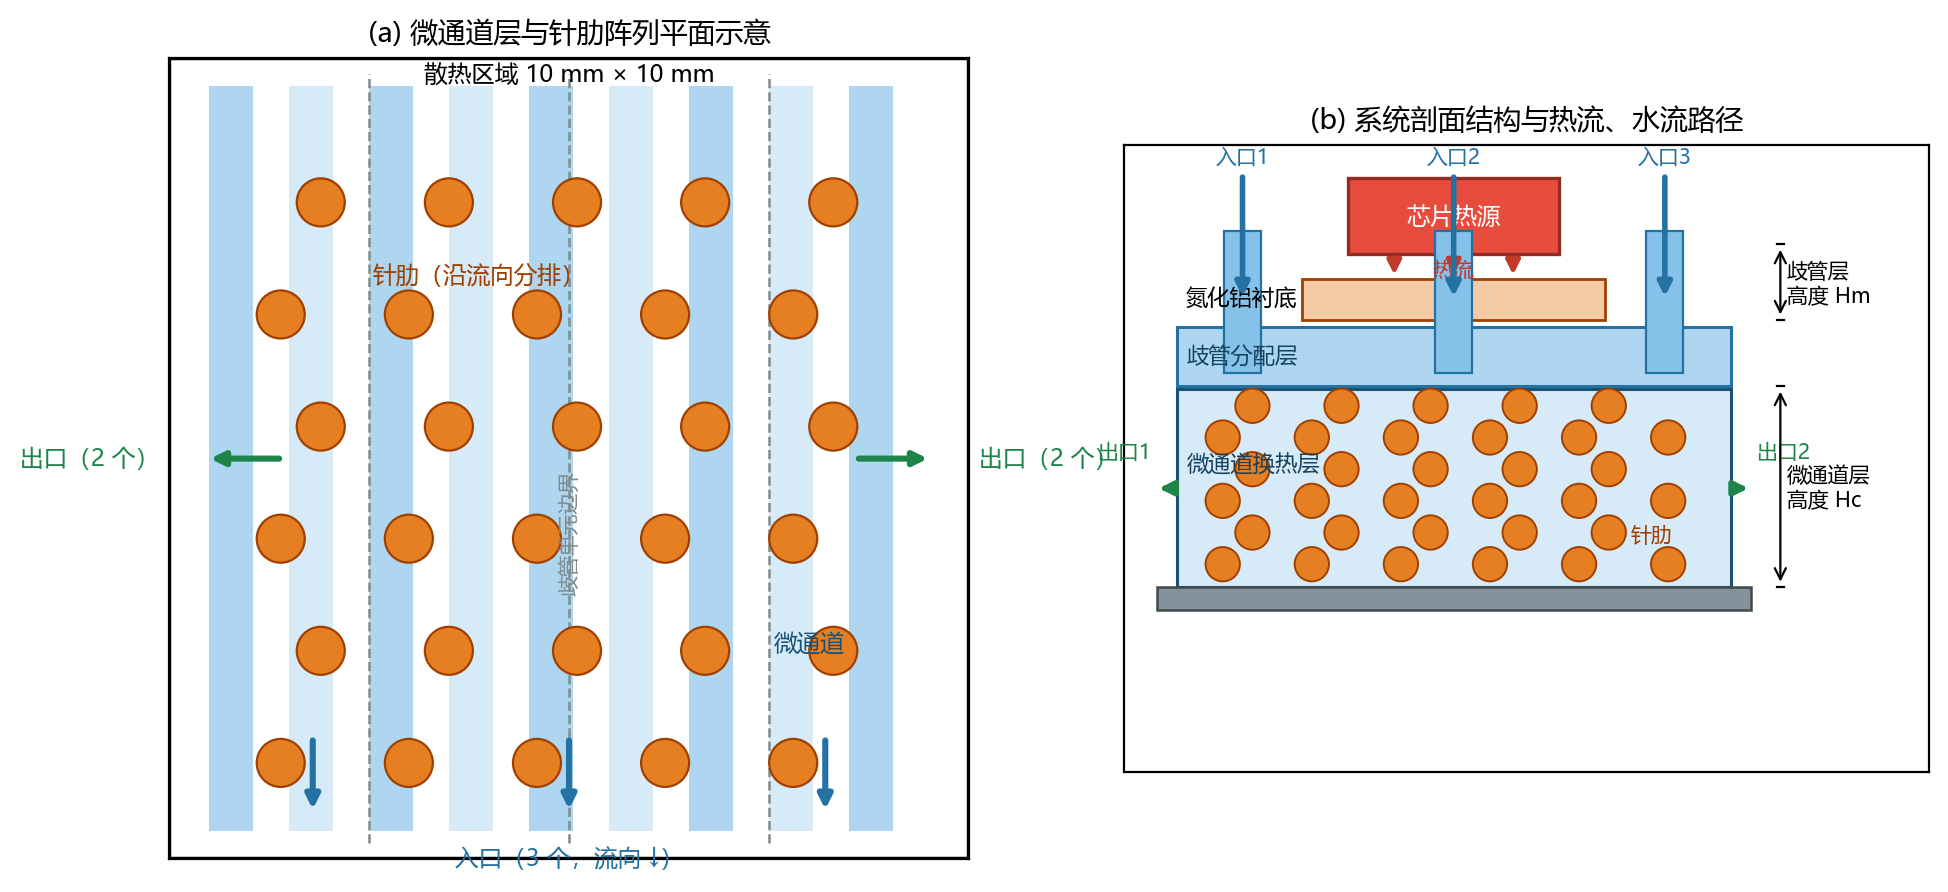
\includegraphics[width=0.92\textwidth]{figs/fig2_structure.png}
  \caption{歧管式微通道热管理系统结构与热流、水流路径示意图}
  \label{fig:structure}
\end{figure}

\subsect{5.1.2\quad 共轭传热控制方程}
流体域的质量、动量和能量守恒为：
\begin{equation}
  \nabla\cdot\mathbf{u} = 0,
  \label{eq:4}
\end{equation}
\begin{equation}
  \rho\,(\mathbf{u}\cdot\nabla)\,\mathbf{u} = -\nabla p + \mu\nabla^2 \mathbf{u} + \rho\,\mathbf{g},
  \label{eq:5}
\end{equation}
\begin{equation}
  \rho\, c_p\, \mathbf{u}\cdot\nabla T_f = \nabla\cdot(k_f\nabla T_f).
  \label{eq:6}
\end{equation}
芯片与氮化铝固体域满足：
\begin{equation}
  \nabla\cdot(k_s\nabla T_s) + q_s''' = 0, \qquad
  q_s''' = \begin{cases}
    5\times 10^{9}, & r \in \Omega_{\mathrm{chip}},\\
    0, & r \in \Omega_{\mathrm{AlN}}.
  \end{cases}
  \label{eq:7}
\end{equation}
流固界面满足温度和法向热流连续：
\begin{equation}
  T_s = T_f, \qquad -k_s\frac{\partial T_s}{\partial n_s} = -k_f\frac{\partial T_f}{\partial n_s}.
  \label{eq:8}
\end{equation}
入口给定 $T_{\mathrm{in}} = 293\ \mathrm{K}$ 和质量流量，出口给定 $p_{\mathrm{out}} = 0\ \mathrm{Pa}$ 表压，固体外侧满足：
\begin{equation}
  -k_s\frac{\partial T_s}{\partial n} = h_{\mathrm{air}}(T_s - T_\infty), \qquad T_\infty = 293\ \mathrm{K}.
  \label{eq:9}
\end{equation}
式（\ref{eq:4}）—（\ref{eq:9}）与由 $(\beta,\lambda,N)$ 决定的流固区域共同构成精确边值问题，其数值求解可参照经典传热与流体力学理论[9]。题设工况与边界条件为：冷却液入口质量流量 1 g/s、入口温度 293 K、出口压力 0 Pa（表压）、外界环境温度 293 K、散热器外侧面对空气自然对流换热系数 10 W/(m$^2$·K)、芯片体热源强度 $5\times10^{9}$ W/m$^3$。下面将式（\ref{eq:4}）—（\ref{eq:9}）降阶为能够显示结构参数作用路径的水力与换热网络。

\subsect{5.1.3\quad 歧管—微通道水力网络}
将换热区沿歧管方向划分为 $J$ 个单元，第 $j$ 条微通道支路流量为 $\dot m_j$。供水歧管和集水歧管中轴向流量分别为 $M_j^s$、$M_j^c$，节点质量守恒为：
\begin{equation}
  M_{j+1}^{s} = M_j^{s} - \dot m_j, \qquad M_{j+1}^{c} = M_j^{c} + \dot m_j, \qquad \sum_{j=1}^{J}\dot m_j = \dot m_\Sigma.
  \label{eq:10}
\end{equation}
更一般地，若把三个入口、两个出口及全部流道视为有向图，节点—边关联矩阵 $B$ 满足：
\begin{equation}
  B\,\mathbf{m}_e = \mathbf{s}, \qquad \mathbf{1}^{\mathrm{T}}\mathbf{s} = 0.
  \label{eq:11}
\end{equation}
第 $j$ 支路两端压差与流量匹配：
\begin{equation}
  p_j^{s} - p_j^{c} = \left[f_c\frac{L_c}{D_{h,c}} + K_v + N\,K_p(\beta, Re_g, \cdots)\right]\frac{\rho u_g^{2}}{2}.
  \label{eq:12}
\end{equation}
水力直径和 Reynolds 数为：
\begin{equation}
  D_h = \frac{4A_f}{P_w}, \qquad Re = \frac{\rho u D_h}{\mu}.
  \label{eq:13}
\end{equation}
若一个歧管单元平面面积为 $A_{pl}$，每排有 $n_\perp$ 根圆柱针肋，则针肋平面占据率与等效孔隙率为：
\begin{equation}
  \phi(\beta, N) = \frac{N\, n_\perp\, \pi\, \beta^{2} w_c^{2}}{4 A_{pl}},
  \label{eq:14}
\end{equation}
\begin{equation}
  \varepsilon = 1 - \phi.
  \label{eq:15}
\end{equation}
在支路流量给定时，针肋区速度尺度满足：
\begin{equation}
  u_g \sim \frac{\dot m_j}{\rho\,\varepsilon\, A_{c0}}.
  \label{eq:16}
\end{equation}
因此 $\beta$ 或 $N$ 增大都会降低孔隙率、提高间隙速度；同时 $K_p$ 随阻塞增强，排数还使损失近似逐排累加。

歧管若近似为宽 $W_m$、高 $H_m = \lambda H_c$ 的矩形流道，则：
\begin{equation}
  A_m = W_m\lambda H_c, \qquad u_m = \frac{\dot m_m}{\rho W_m\lambda H_c}, \qquad D_{h,m} = \frac{2W_m\lambda H_c}{W_m + \lambda H_c}.
  \label{eq:17}
\end{equation}
宽浅层流矩形歧管和局部惯性损失的尺度分别为：
\begin{equation}
  \Delta p_{m,f} \sim \frac{\mu L_m \dot V_m}{W_m H_m^{3}} \propto \lambda^{-3}, \qquad
  \Delta p_{m,\mathrm{loc}} \sim K_m\frac{\rho u_m^{2}}{2} \propto \lambda^{-2}.
  \label{eq:18}
\end{equation}
由此，在题给结构域、总流量固定且不发生旁路拓扑变化时，可判断：
\begin{equation}
  \frac{\partial \Delta p}{\partial \beta} > 0, \qquad \Delta_N \Delta p > 0, \qquad
  \frac{\partial \Delta p}{\partial \lambda} < 0.
  \label{eq:19}
\end{equation}
这里 $\Delta_N \Delta p = \Delta p(N + 2) - \Delta p(N)$。式（\ref{eq:19}）给的是有明确前提的物理趋势，不是脱离具体几何的无条件定理。

\subsect{5.1.4\quad 水侧换热网络与热阻}
第 $j$ 支路的混合平均水温满足：
\begin{equation}
  \dot m_j c_p \frac{dT_{b,j}}{dx} = h_j P_{w,j}\,(T_{w,j} - T_{b,j}).
  \label{eq:20}
\end{equation}
若单元内壁温近似为常数，积分得：
\begin{equation}
  T_{\mathrm{out},j} = T_{w,j} - (T_{w,j} - T_{\mathrm{in},j})\,e^{-NTU_j}, \qquad
  NTU_j = \frac{h_j A_{\mathrm{wet},j}}{\dot m_j c_p}.
  \label{eq:21}
\end{equation}
若针肋贯穿微通道高度，湿润面积可写为：
\begin{equation}
  A_{\mathrm{wet}} = A_{w0} + N\,n_\perp\left(\pi\beta w_c H_c - \nu_b\frac{\pi\beta^{2} w_c^{2}}{4}\right).
  \label{eq:22}
\end{equation}
其中 $\nu_b$ 表示需要扣除的有效受热投影面数，取决于针肋与一侧或两侧壁面的连接形式。对流换热系数为：
\begin{equation}
  h = \frac{k_f Nu}{D_{h,c}}, \qquad
  Nu = F_{Nu}\left(Re_g, Pr, \beta, N, \frac{s_x}{d_p}, \frac{s_y}{d_p}, \frac{H_c}{w_c}\right).
  \label{eq:23}
\end{equation}
以芯片最高温度定义热阻：
\begin{equation}
  R_{th} = \frac{T_{\max} - T_{\mathrm{in}}}{Q}
         = R_{\mathrm{chip,gen}} + R_{\mathrm{spread}} + R_{\mathrm{conv}} + R_{\mathrm{fluid,mal}}.
  \label{eq:24}
\end{equation}
其中：
\begin{equation}
  R_{\mathrm{conv}} = \frac{1}{h A_{\mathrm{wet}}} = \frac{D_{h,c}}{k_f\, Nu\, A_{\mathrm{wet}}}.
  \label{eq:25}
\end{equation}
对 $x \in \{\beta, N\}$ 求对数灵敏度：
\begin{equation}
  \frac{\partial \ln R_{\mathrm{conv}}}{\partial x}
  = \frac{\partial \ln D_{h,c}}{\partial x} - \frac{\partial \ln Nu}{\partial x} - \frac{\partial \ln A_{\mathrm{wet}}}{\partial x}.
  \label{eq:26}
\end{equation}
式（\ref{eq:26}）揭示了热阻非单调性的根源：针肋初期增加时，$Nu \cdot A_{\mathrm{wet}}$ 的增长占优，热阻下降；继续加粗或加密后，尾迹滞流、流量重分配与有效面积缩减占优，热阻收益饱和甚至反弹。歧管深度通过改变支路流量和射流速度间接作用于热阻，因此守恒律本身不能保证 $R_{th}$ 对 $\lambda$ 单调。

\subsect{5.1.5\quad 温度非均匀性}
附件没有公布无量纲温度非均匀性的原始基准。机理层以等面积采样温度的标准差型指标说明其来源：
\begin{equation}
  U_T = \frac{\sigma_T}{\Theta_{\mathrm{ref}}}, \qquad
  \sigma_T = \sqrt{\frac{1}{M}\sum_{i=1}^{M}(T_i - \bar T)^{2}}.
  \label{eq:27}
\end{equation}
其中 $\Theta_{\mathrm{ref}} > 0$ 为固定温差基准。数值层直接学习附件给出的 $U_T^{*}$，不以式（\ref{eq:27}）擅自替换原始指标。

定义支路流量变异系数：
\begin{equation}
  C_m = \frac{\sqrt{\frac{1}{J}\sum_{j=1}^{J}(\dot m_j - \bar m)^{2}}}{\bar m}, \qquad
  \bar m = \frac{\dot m_\Sigma}{J}.
  \label{eq:28}
\end{equation}
局部温升近似为：
\begin{equation}
  T_i - T_{\mathrm{in}} \simeq Q_i R_{s,i} + \frac{Q_i}{h_i A_i} + \frac{Q_{\mathrm{up},i}}{\dot m_i c_p}.
  \label{eq:29}
\end{equation}
令 $\dot m_i = \bar m(1 + \delta_i)$、$h_i \propto \dot m_i^{a_i}$，对式（\ref{eq:29}）作一阶展开可得：
\begin{equation}
  T_i - \bar T \simeq -\left(a_i\frac{Q_i}{\bar h_i A_i} + \frac{Q_{\mathrm{up},i}}{\bar m c_p}\right)\delta_i + \delta_{T_g,i}.
  \label{eq:30}
\end{equation}
因此温度离散度的一阶量级与流量不均匀 $C_m$ 正相关，并叠加固体扩散路径和针肋尾迹造成的局部差异。适度加深歧管有利于减小歧管压力梯度和 $C_m$，但过深又可能降低射流速度；适量针肋能均化换热，过粗或过多则会制造低速区。因此 $U_T$ 对三参数均可能存在中间最优。

\subsect{5.1.6\quad 三指标作为综合评价依据的合理性}
热阻决定最高温度、压降决定泵功、温度非均匀性关联受约束材料的热应力量级：
\begin{equation}
  T_{\max} = T_{\mathrm{in}} + Q\, R_{th},
  \label{eq:31}
\end{equation}
\begin{equation}
  P_{\mathrm{pump}} = \frac{\Delta p\, \dot V}{\eta_p},
  \label{eq:32}
\end{equation}
\begin{equation}
  \sigma_{th} \sim \frac{E\,\alpha_T}{1 - \nu}\,\Delta T.
  \label{eq:33}
\end{equation}
故三指标分别衡量绝对温度水平、流动能耗与空间热应力。它们在数学上互不决定：相同最高温度可以对应不同温度场，相同温度分布也可以需要不同泵功。删去任一项，都可能把过热、高能耗或存在严重热点的结构误判为优良结构。

\subsect{5.1.7\quad 样本主效应对机理的验证}
为避免拓扑差异混淆，图 \ref{fig:maineff} 只统计 80 个带针肋完整因子样本，并对另外两个变量取平均。

从 $\beta = 0.10$ 增至 0.20，热阻和非均匀性分别下降约 1.98\% 和 2.50\%，压降增加约 7.07\%；继续增至 0.30，压降骤增约 28.21\%，热阻和非均匀性分别反弹约 0.91\% 和 2.79\%。这与``换热面积/扰动强化—堵塞/尾迹损失''的竞争一致。

$\lambda$ 从 3.0 增至 4.5 时，压降下降约 32.15\%，验证了式（\ref{eq:18}）的尺度判断；热阻总体增加约 1.94\%，均匀性在 $\lambda = 3.5$ 附近最好，说明压力分配改善与冲击换热减弱同时存在。

$N$ 从 2 增至 10 时，热阻下降约 2.18\%，但压降增加约 30.90\%，且热阻边际收益递减；非均匀性在 4 排最小，随后因尾迹累积和支路重分配而恶化。主效应只能显示平均趋势，$\beta\lambda$、$\beta N$、$\lambda N$ 交互作用仍需代理模型定量识别。

\begin{figure}[htbp]
  \centering
  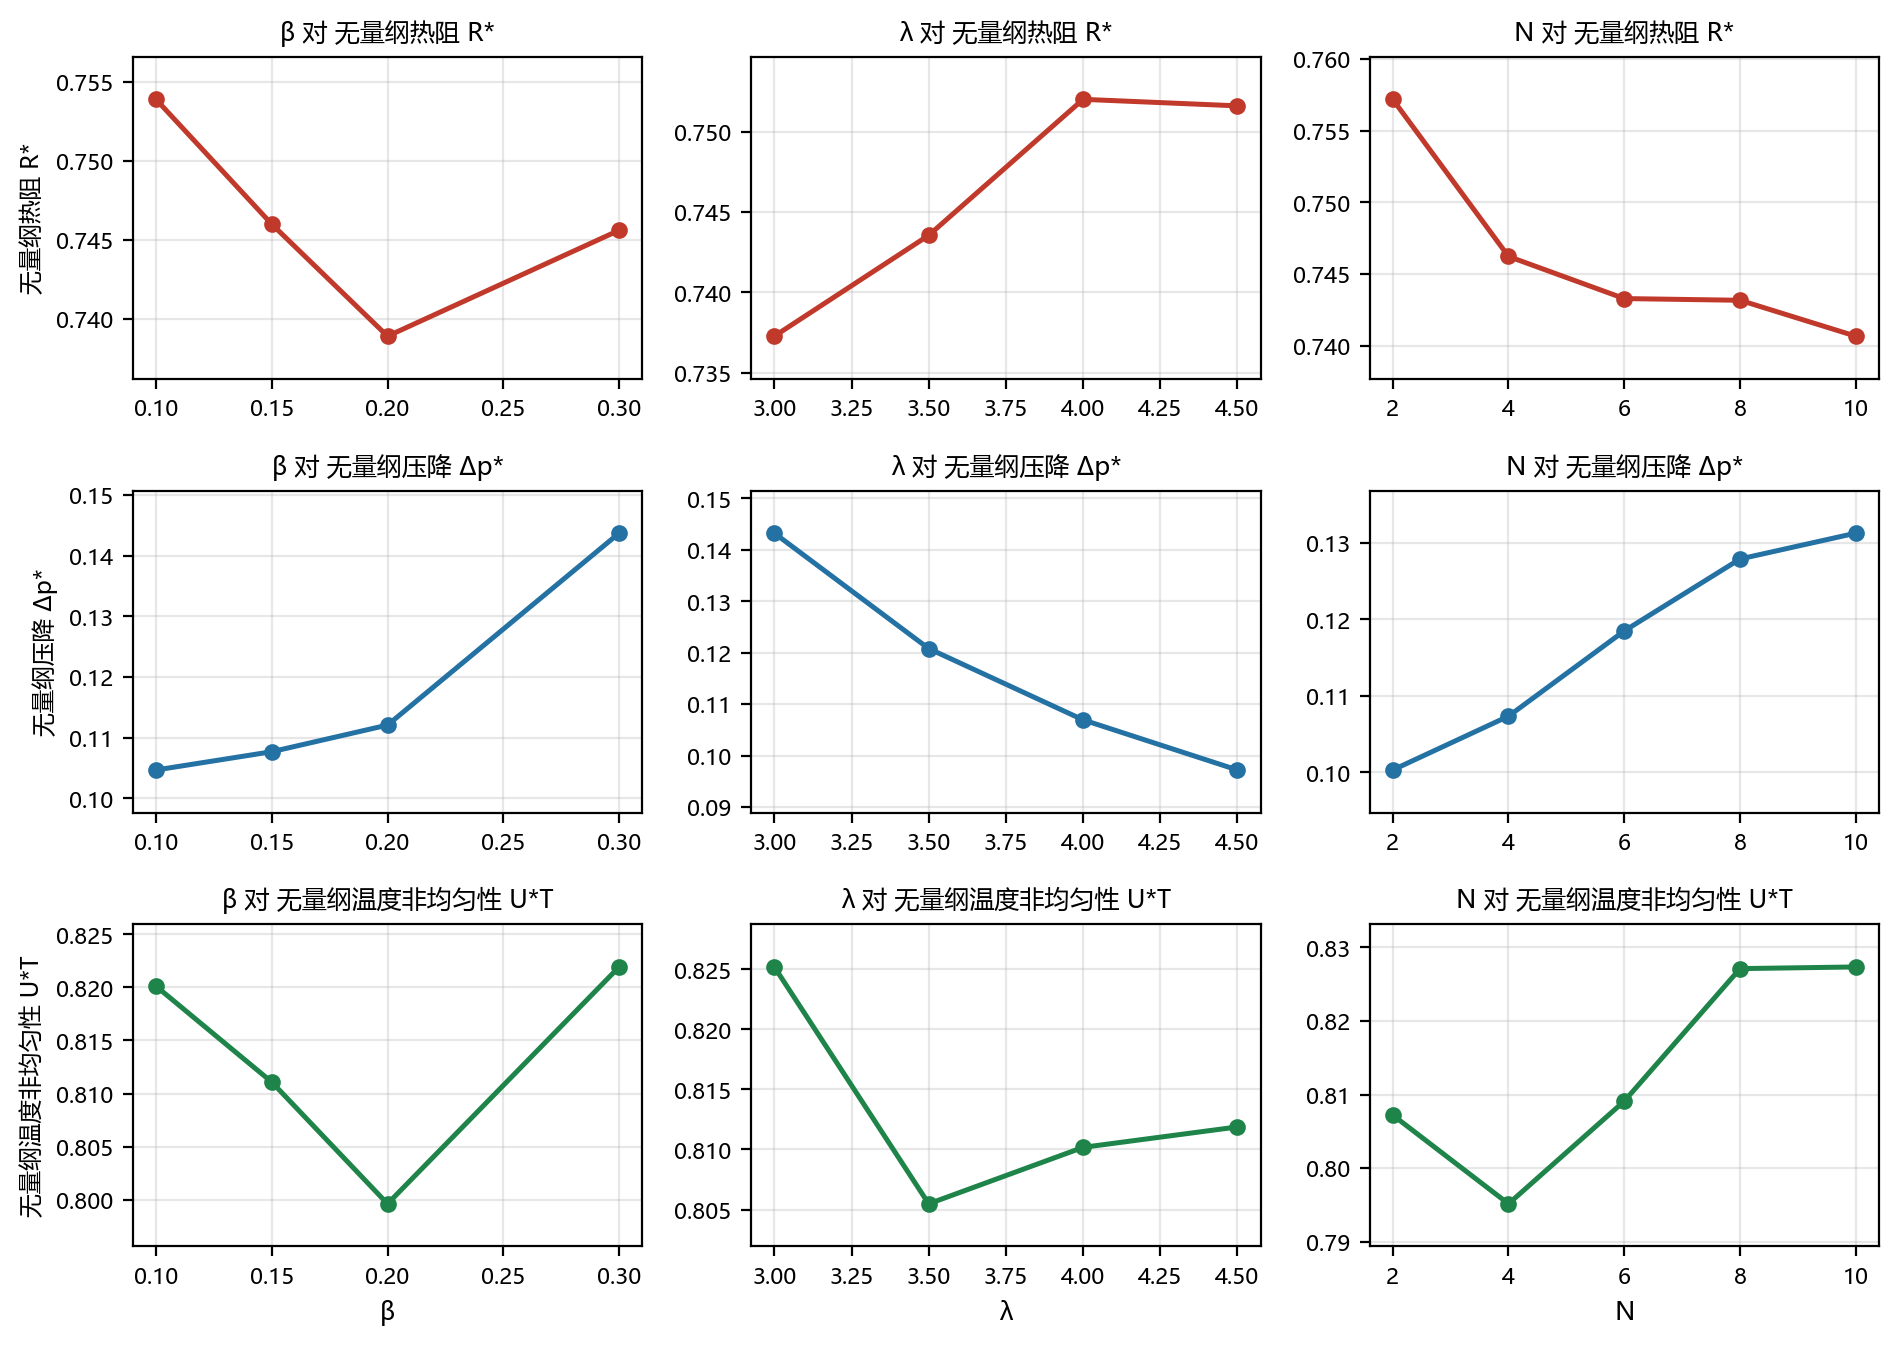
\includegraphics[width=0.9\textwidth]{figs/fig3_maineffects.png}
  \caption{结构参数对三项性能指标的主效应（80 个带针肋样本，其余两变量取平均）}
  \label{fig:maineff}
\end{figure}

\subsect{5.2\quad 条件代理模型}
\subsect{5.2.1\quad 数据结构与拓扑分组}
附件 2 共 84 个样本，其中：80 个带针肋点构成 $4 \times 4 \times 5$ 完整因子网格，$\beta \in \{0.10, 0.15, 0.20, 0.30\}$、$\lambda \in \{3, 3.5, 4, 4.5\}$、$N \in \{2, 4, 6, 8, 10\}$；4 个无针肋点满足 $\beta = 0$、$N = 0$，仅改变参数 $\lambda$。有无针肋是实体拓扑改变，而不是普通连续变化。若强行用一个三变量光滑面连接全部样本，模型会在 $\beta \to 0$、$N > 0$ 等不存在的几何上产生伪预测。因此定义条件代理模型：
\begin{equation}
  \hat y_k(\mathbf{x}) = \begin{cases}
    g_{k,0}(\lambda), & \beta = 0,\ N = 0,\\
    g_{k,p}(\beta,\lambda,N), & \beta > 0,\ N \geq 2.
  \end{cases}
  \label{eq:34}
\end{equation}
无针肋组只有 4 点，仅用一维二次曲线表示基准趋势；所有推荐方案均位于带针肋完整数据域。

\subsect{5.2.2\quad 候选模型与标准化}
比较二次响应面、三次响应面和高斯过程回归。三次响应面写为：
\begin{equation}
  g_{k,p} = a_{k,0} + \sum_{1\leq i+j+l\leq 3} a_{k,ijl}\, z_\beta^{i}\, z_\lambda^{j}\, z_N^{l}.
  \label{eq:35}
\end{equation}
标准化变量为：
\begin{equation}
  z_\beta = \frac{\beta - 0.1875}{0.073951}, \qquad
  z_\lambda = \frac{\lambda - 3.75}{0.559017}, \qquad
  z_N = \frac{N - 6}{2.828427}.
  \label{eq:36}
\end{equation}
标准化改善多项式设计矩阵的数值条件；三次项能够表达图 \ref{fig:maineff} 中的转折、曲率及二阶交互随第三变量变化的现象。为抑制极弱病态性，对系数施加 $10^{-10}$ 的 Ridge 正则，其量级足够小，不改变响应面的实际拟合[10]。

\subsect{5.2.3\quad 交叉验证与模型选择}
在 80 个带针肋点上实施 5 次重复的 5 折交叉验证。评价指标为：
\begin{equation}
  R^{2} = 1 - \frac{\sum_i (y_i - \hat y_i)^{2}}{\sum_i (y_i - \bar y)^{2}}, \qquad
  RMSE = \sqrt{\frac{1}{n}\sum_i (y_i - \hat y_i)^{2}}, \qquad
  NRMSE = \frac{RMSE}{y_{\max} - y_{\min}}.
  \label{eq:37}
\end{equation}
图 \ref{fig:cvparity} 给出一次确定性五折留出预测的样本—预测一致性，图 \ref{fig:modelcmp} 汇总重复交叉验证的候选模型误差。

\begin{figure}[htbp]
  \centering
  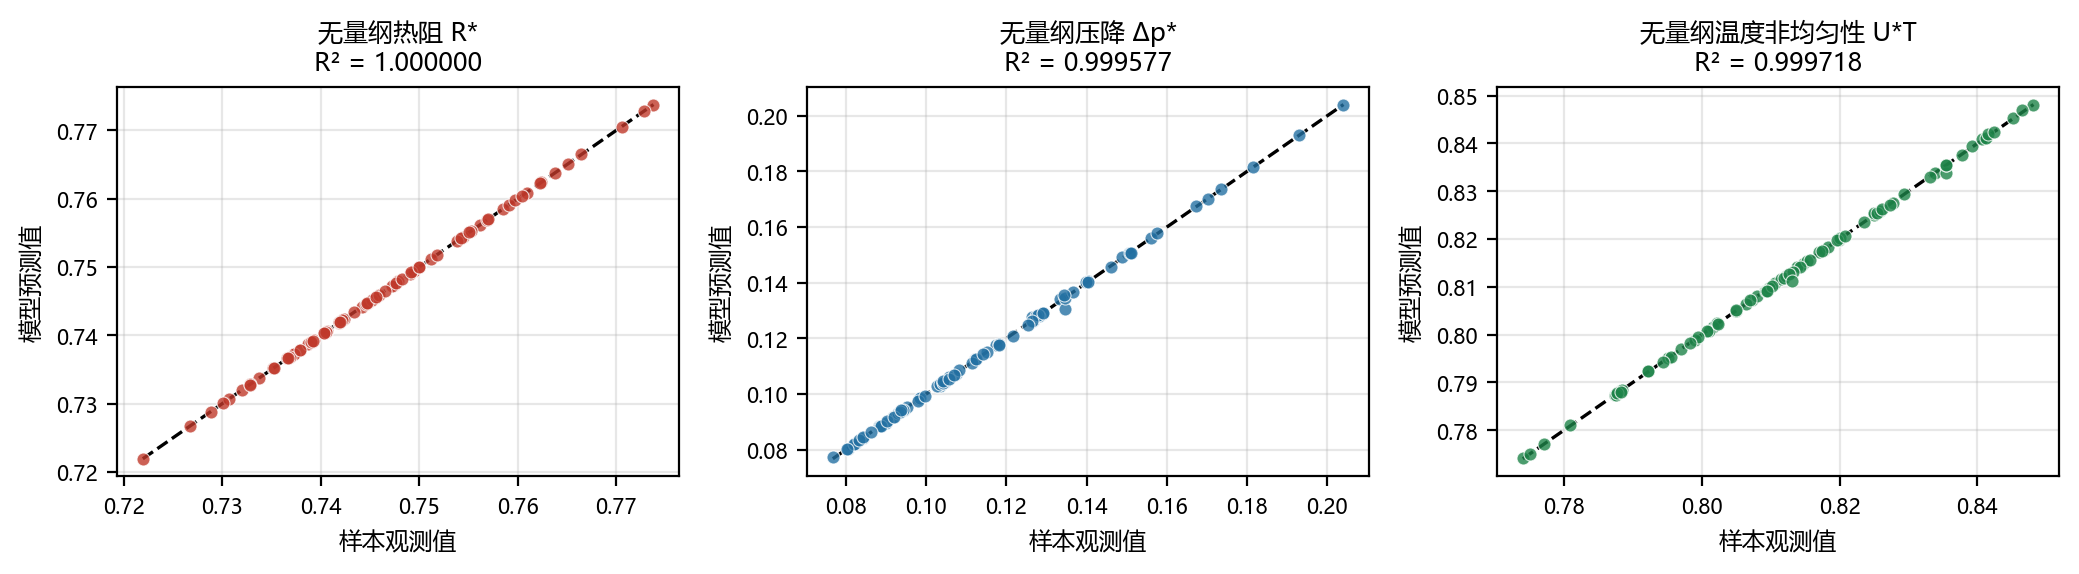
\includegraphics[width=0.93\textwidth]{figs/fig4_cv_parity.png}
  \caption{三次响应面一次确定性 5 折交叉验证的样本—预测一致性}
  \label{fig:cvparity}
\end{figure}

\begin{figure}[htbp]
  \centering
  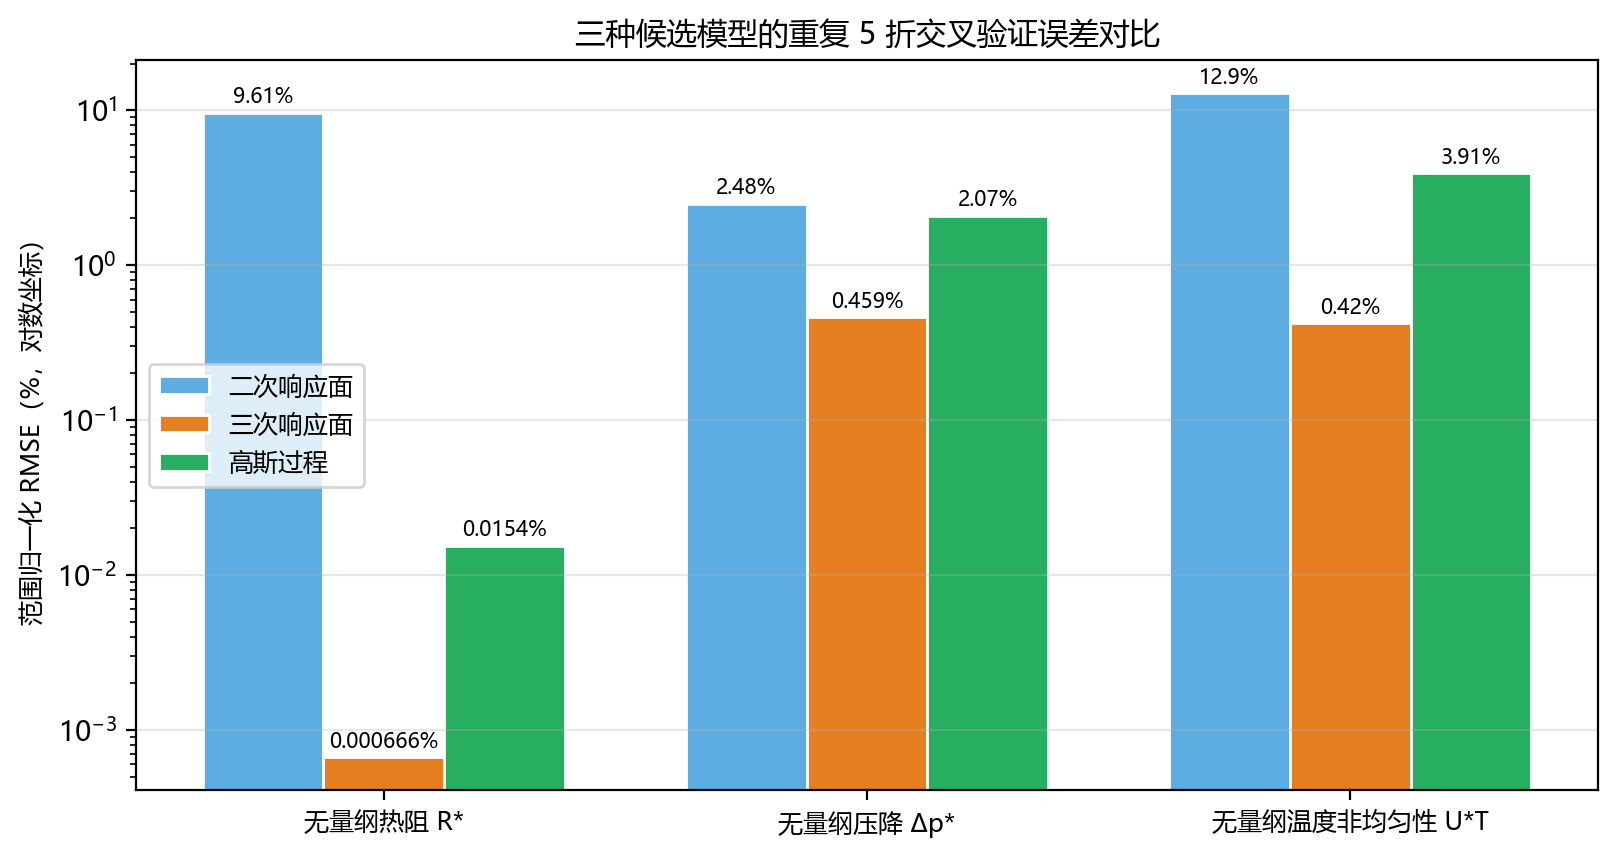
\includegraphics[width=0.82\textwidth]{figs/fig5_model_cmp.png}
  \caption{三种候选模型重复 5 折交叉验证误差对比（5 次重复）}
  \label{fig:modelcmp}
\end{figure}

\begin{table}[htbp]
  \centering
  \caption{选定三次响应面的重复交叉验证性能}
  \label{tab:cv}
  \begin{tabular}{lccccc}
    \toprule
    指标 & $R^{2}$ & MAE & RMSE & 范围归一化 RMSE \\
    \midrule
    无量纲热阻 & 1.000000 & $2.910\times10^{-7}$ & $3.455\times10^{-7}$ & 0.000666\% \\
    无量纲压降 & 0.999555 & 0.000246 & 0.000585 & 0.459\% \\
    无量纲温度非均匀性 & 0.999699 & 0.000158 & 0.000311 & 0.420\% \\
    \bottomrule
  \end{tabular}
\end{table}

三次响应面在三项输出上均优于二次响应面和高斯过程[10-11]，且连续可微、系数可导出，适合后续全域搜索、局部灵敏度及误差传播。热阻的近零误差说明该响应在给定网格内几乎完全符合低阶多项式结构；这不意味着模型在样本域外仍然精确，故后续禁止外推。

\subsect{5.2.4\quad 响应面解释}
固定 $N = 4$ 的三项响应如图 \ref{fig:response}。热阻在较小 $\lambda$ 和中等 $\beta$ 一带较低；压降随 $\lambda$ 增大明显降低，并在 $\beta$ 过大时迅速上升；非均匀性在 $\beta \approx 0.22$、较大 $\lambda$ 附近形成低谷。三幅图的最优区域不重合，直观证明单目标最优不可能同时满足全部要求。

\begin{figure}[htbp]
  \centering
  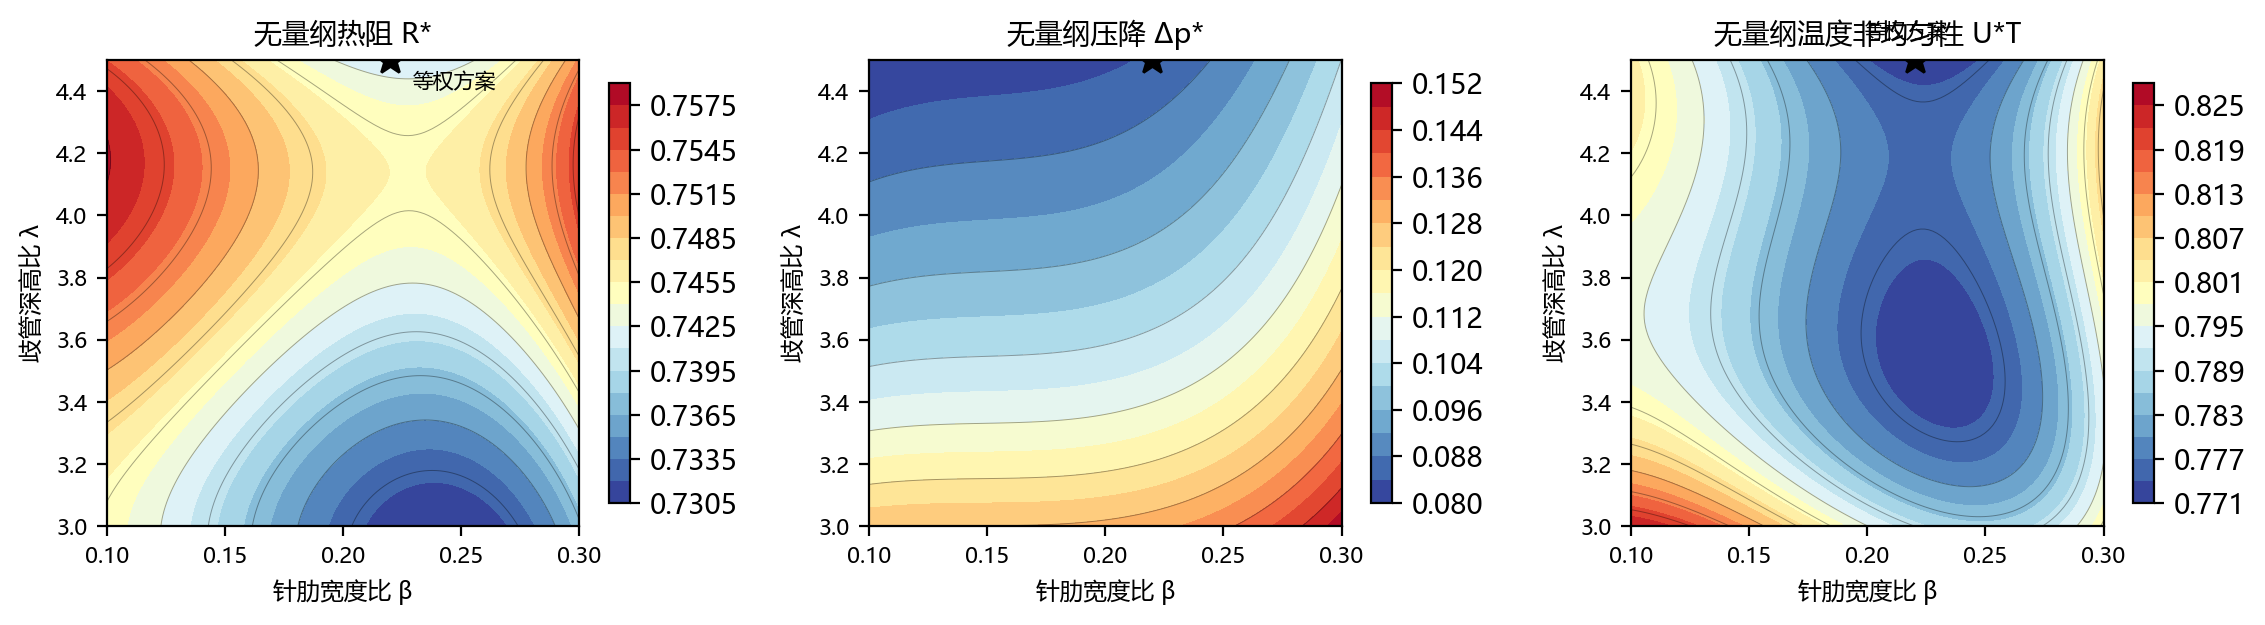
\includegraphics[width=0.95\textwidth]{figs/fig6_response.png}
  \caption{固定 $N = 4$ 时三项性能指标的响应面}
  \label{fig:response}
\end{figure}

\subsect{5.3\quad 三目标优化与综合方案}
\subsect{5.3.1\quad 优化模型}
针对三目标结构优化问题，采用加权和与 Pareto 支配相结合的方法求解[12]。建立三目标最小化模型：
\begin{equation}
  \min_{\beta,\lambda,N}\ \left[\hat R^{*}(\beta,\lambda,N),\ \widehat{\Delta p}^{\,*}(\beta,\lambda,N),\ \hat U_T^{*}(\beta,\lambda,N)\right].
  \label{eq:38}
\end{equation}
约束为：
\begin{equation}
  0.10 \leq \beta \leq 0.30, \qquad 3 \leq \lambda \leq 4.5, \qquad
  N \in \{2, 4, 6, 8, 10\}.
  \label{eq:39}
\end{equation}
$N$ 是离散可制造变量，不能取 5.37 排。对连续变量采用 $\Delta\beta = 0.001$、$\Delta\lambda = 0.01$ 的规则网格，并枚举五种排数，共评价约 15 万个带针肋方案。确定性网格搜索不依赖随机初值，分辨率足以支持 $\beta$ 报告到三位小数、$\lambda$ 报告到两位小数。

\subsect{5.3.2\quad Pareto 支配与指标归一化}
若方案 $\mathbf{x}_a$ 在三项目标上均不差于 $\mathbf{x}_b$，且至少一项严格更优，则称 $\mathbf{x}_a$ 支配 $\mathbf{x}_b$。所有不被其他可行方案支配的点构成 Pareto 集。不同指标的数值跨度不同，先按题给全部样本的实际极值归一化：
\begin{equation}
  s_k(\mathbf{x}) = \frac{\hat y_k(\mathbf{x}) - y_k^{\min}}{y_k^{\max} - y_k^{\min}}, \qquad k = 1,\,2,\,3.
  \label{eq:40}
\end{equation}
题目没有声明指标优先级，因此综合方案采用等权损失：
\begin{equation}
  L_{\mathrm{eq}}(\mathbf{x}) = \frac{s_1(\mathbf{x}) + s_2(\mathbf{x}) + s_3(\mathbf{x})}{3}.
  \label{eq:41}
\end{equation}
没有采用熵权法：指标样本离散程度是数据性质，不等于使用方的价值偏好。等权表示``当前没有证据认为某一指标更重要''，并将在问题四中显式改变权重。图 \ref{fig:pareto} 展示支持型 Pareto 前沿。降低热阻通常伴随压降上升；低压降区需要较少针肋，却不能同时取得最低热阻；温度非均匀性最优区位于中间折中段。

\begin{figure}[htbp]
  \centering
  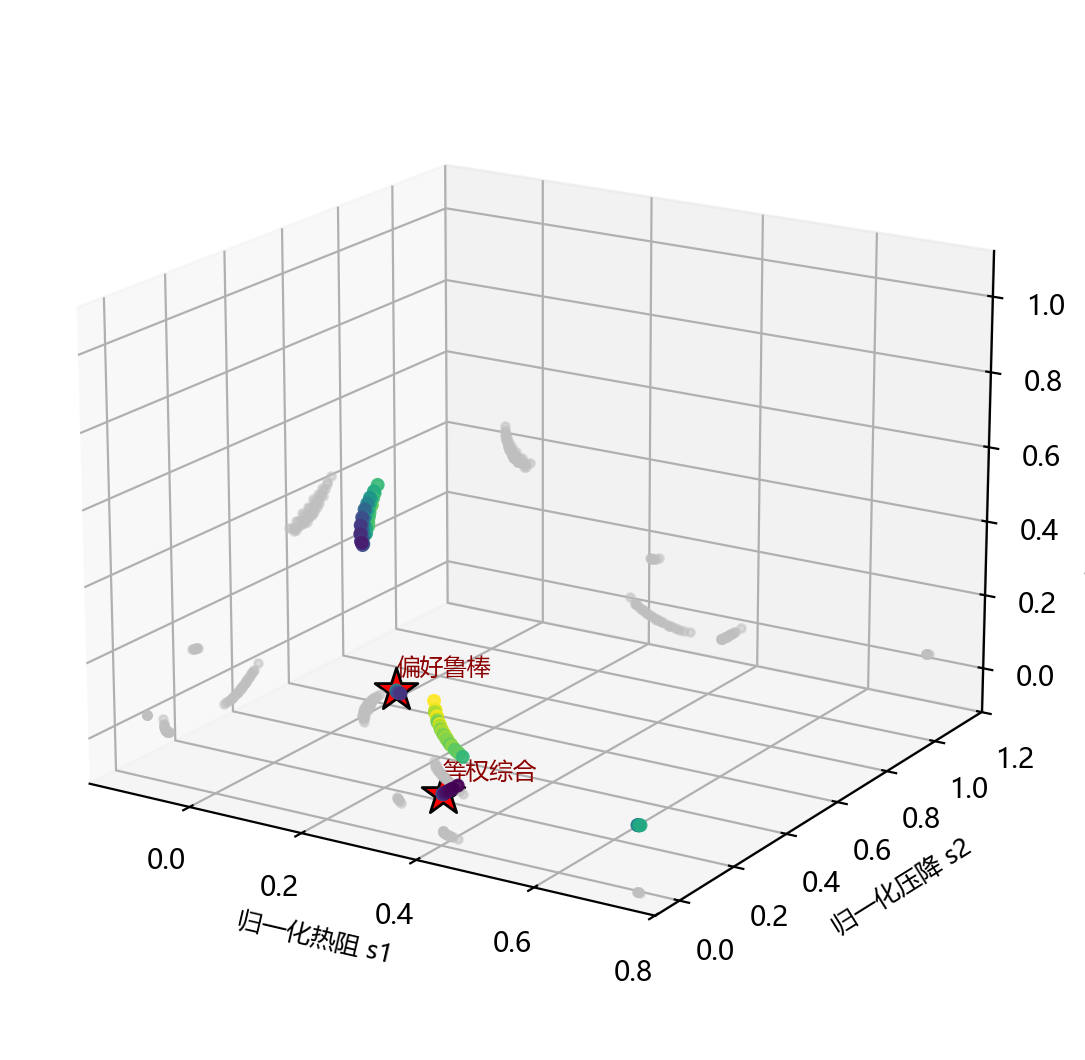
\includegraphics[width=0.8\textwidth]{figs/fig7_pareto.png}
  \caption{支持型 Pareto 前沿（0.05 权重网格扫描，115 个方案）}
  \label{fig:pareto}
\end{figure}

\subsect{5.3.3\quad 优化结果}
等权综合推荐为：
\begin{equation}
  (\beta,\ \lambda,\ N) = (0.220,\ 4.50,\ 4).
  \label{eq:42}
\end{equation}
该方案与均匀性优先方案接近，说明温度均匀性低谷与综合折中区域重合；其压降接近低压区，同时避免 2 排方案较高的热阻。以到归一化理想点的加权欧氏距离进行独立交叉检查，得到 $(0.224, 4.50, 6)$，仍落在``$\beta$ 约 0.22、$\lambda$ 取上界、$N$ 为 4—6''的同一区域，且与严格最优点的距离差异小于 $10^{-5}$，说明结论不依赖唯一一种综合准则。

\begin{table}[htbp]
  \centering
  \caption{不同决策准则下的参数配置与性能指标对比}
  \label{tab:criteria}
  \begin{tabular}{lcccccc}
    \toprule
    决策准则 & $\beta$ & $\lambda$ & $N$ & 热阻 & 压降 & 非均匀性 \\
    \midrule
    热阻优先 (0.8, 0.1, 0.1) & 0.228 & 3.17 & 10 & 0.720555 & 0.151744 & 0.813938 \\
    压降优先 (0.1, 0.8, 0.1) & 0.223 & 4.50 & 2 & 0.759933 & 0.076083 & 0.779019 \\
    均匀性优先 (0.1, 0.1, 0.8) & 0.224 & 4.50 & 4 & 0.741114 & 0.085117 & 0.771783 \\
    等权综合推荐 & 0.220 & 4.50 & 4 & 0.741183 & 0.084698 & 0.771878 \\
    等权理想点距离 & 0.224 & 4.50 & 6 & 0.734381 & 0.097795 & 0.790194 \\
    \bottomrule
  \end{tabular}
\end{table}

\subsect{5.4\quad 偏好变化与偏好鲁棒设计}
\subsect{5.4.1\quad 权重变化的影响}
令权重属于三维单纯形：
\begin{equation}
  \mathcal{W} = \left\{w : w_k \geq 0,\ \sum_{k=1}^{3} w_k = 1\right\}, \qquad
  L(\mathbf{x}, w) = w^{\mathrm{T}} s(\mathbf{x}).
  \label{eq:43}
\end{equation}
图 \ref{fig:weights} 将五类典型方案的归一化损失画在同一坐标上。热阻优先方案显著牺牲压降；压降优先方案牺牲热阻；4 排方案在非均匀性上占优；6 排理想点方案以中等压降换取更低热阻。权重改变不是数值扰动，而是评价标准改变，最优方案沿 Pareto 前沿迁移是合理现象。

\begin{figure}[htbp]
  \centering
  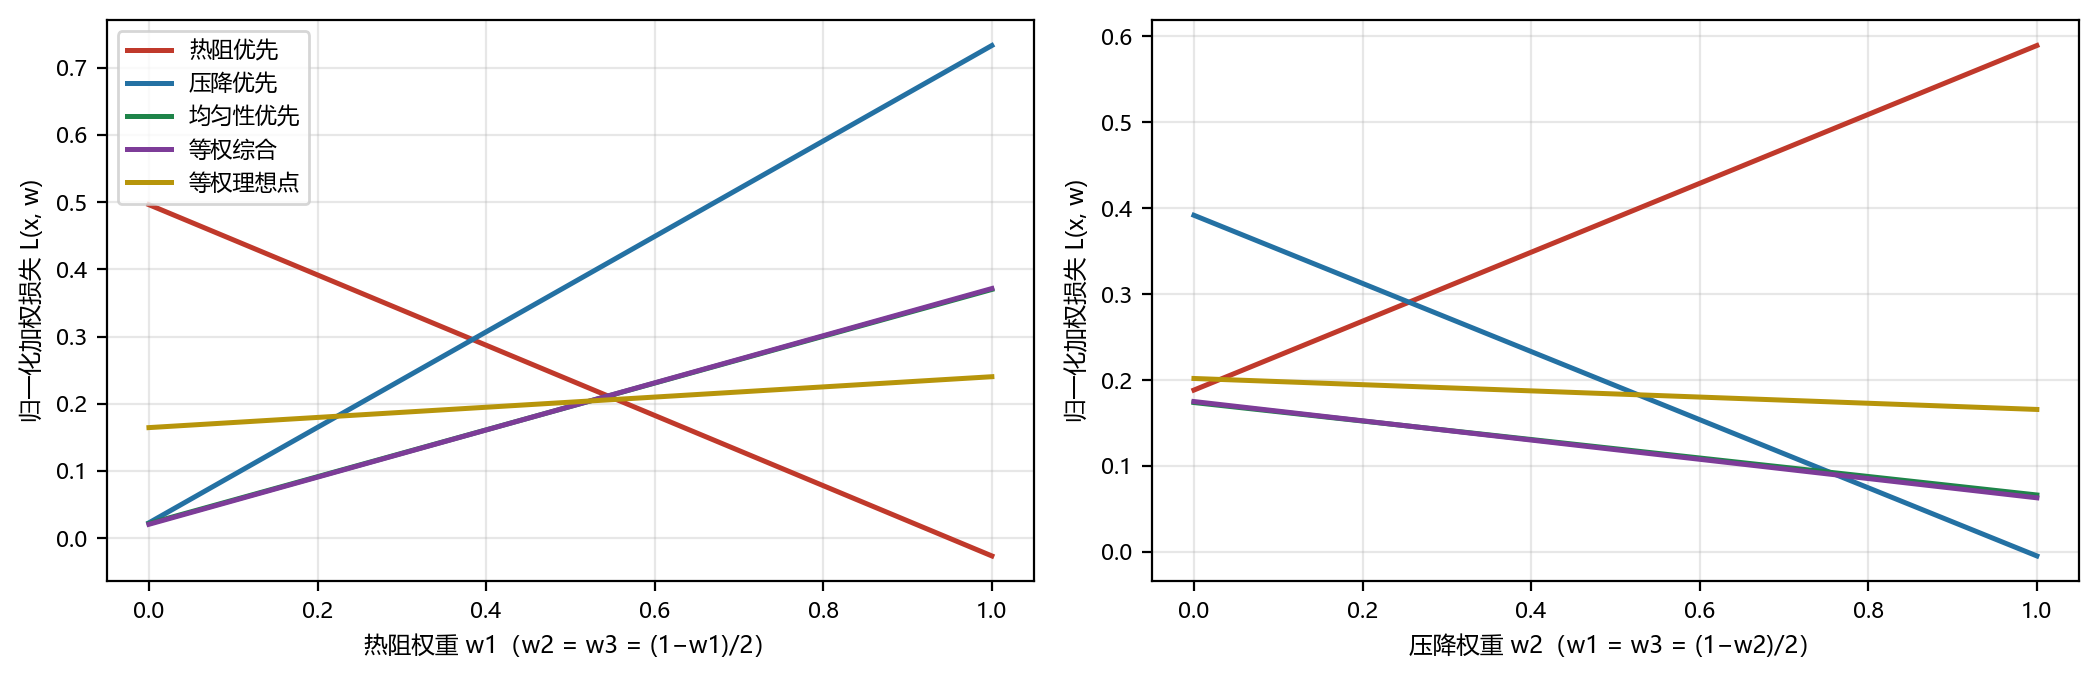
\includegraphics[width=0.93\textwidth]{figs/fig8_weights.png}
  \caption{不同应用偏好下五种典型方案的归一化加权损失}
  \label{fig:weights}
\end{figure}

\subsect{5.4.2\quad 最小最大后悔模型}
若应用偏好尚未确定，只比较平均加权得分会掩盖某些合法权重下的严重失配。定义方案 $\mathbf{x}$ 在权重 $w$ 下的后悔值[13]：
\begin{equation}
  \mathrm{Regret}(\mathbf{x}, w) = L(\mathbf{x}, w) - \min_{\mathbf{x}'\in P} L(\mathbf{x}', w),
  \label{eq:44}
\end{equation}
其中 $P$ 为支持型 Pareto 候选集。选择最小最大后悔方案：
\begin{equation}
  \mathbf{x}_{\mathrm{rob}} = \arg\min_{\mathbf{x}\in P}\ \max_{w\in\mathcal{W}}\ \mathrm{Regret}(\mathbf{x}, w).
  \label{eq:45}
\end{equation}
计算时以 0.05 步长扫描权重以构造 115 个支持型 Pareto 方案，再以 0.01 步长在完整权重单纯形上评价后悔。结果为：
\begin{equation}
  (\beta,\ \lambda,\ N) = (0.226,\ 4.50,\ 6),
  \label{eq:46}
\end{equation}
性能为：
\begin{equation}
  (R^{*},\ \Delta p^{*},\ U_T^{*}) = (0.734274,\ 0.098231,\ 0.790195),
  \label{eq:47}
\end{equation}
最大后悔值为 0.270865。该数是归一化加权损失之差，不是百分比。图 \ref{fig:regret} 中偏好鲁棒方案处于最大后悔值下包络。它相对等权 4 排方案降低热阻，但提高压降与非均匀性；其价值不是``三项性能都更好''，而是在热阻、泵功与均匀性偏好发生切换时控制最坏决策损失。严格地说，该结论在所枚举权重网格与支持型 Pareto 候选集上成立，不宣称对连续无限权重空间给出解析全局证明。

\begin{figure}[htbp]
  \centering
  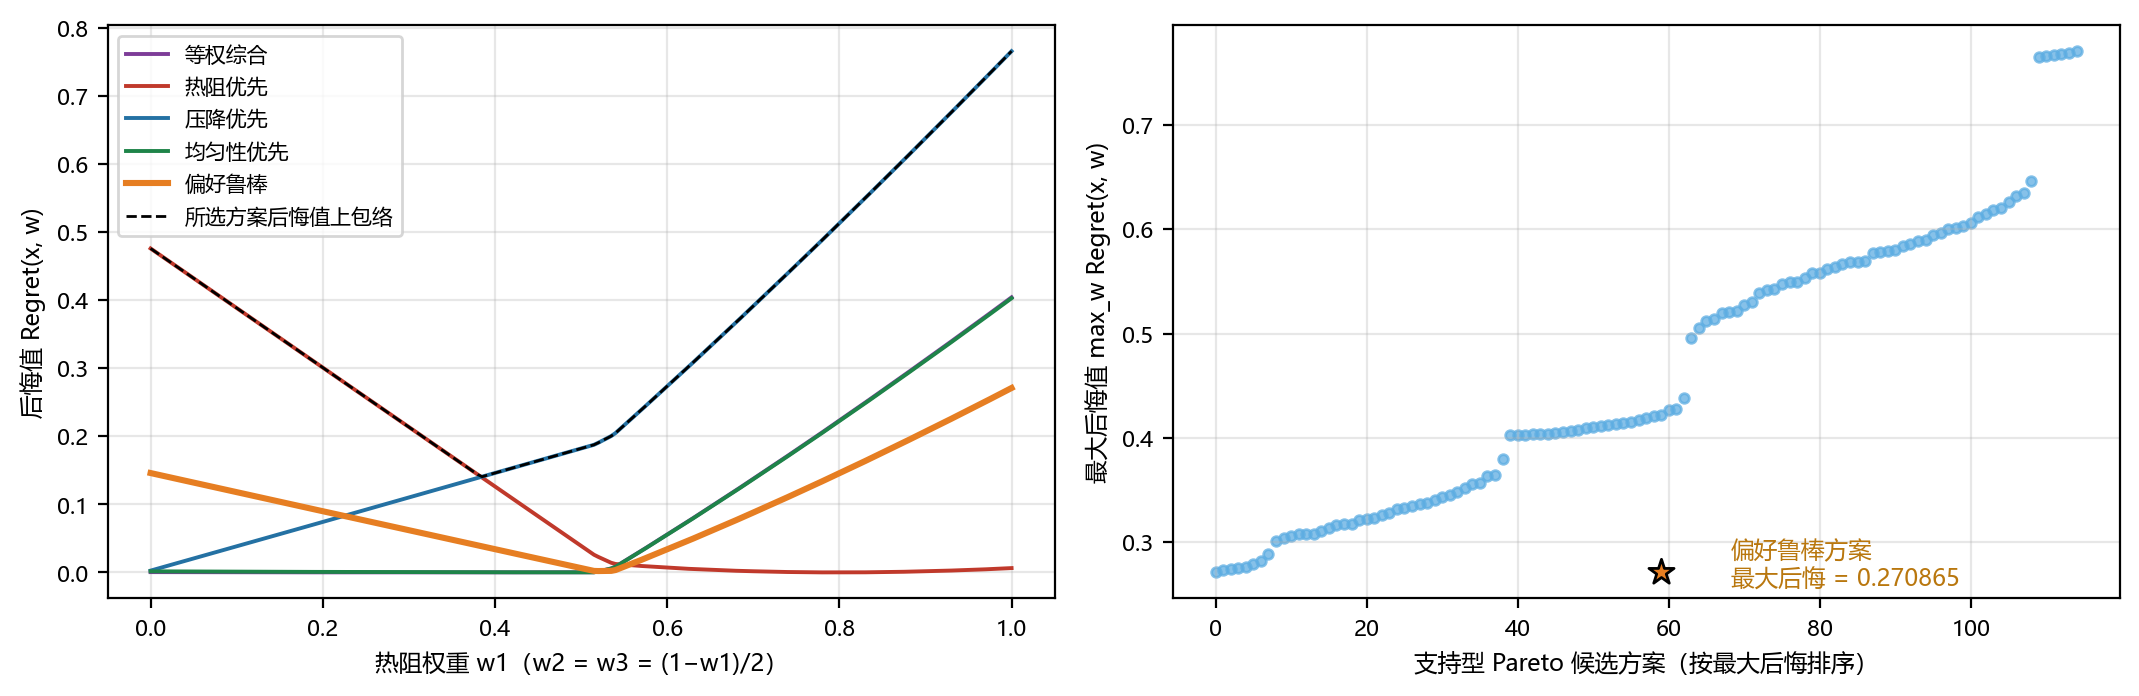
\includegraphics[width=0.95\textwidth]{figs/fig9_regret.png}
  \caption{最小最大后悔分析：左为后悔曲线切片，右为全部候选方案的最大后悔值}
  \label{fig:regret}
\end{figure}

\subsect{5.5\quad 制造误差与运行波动}
\subsect{5.5.1\quad 局部弹性系数}
对连续参数 $x_j \in \{\beta, \lambda\}$，定义无量纲局部弹性：
\begin{equation}
  E_{kj} = \frac{\partial \hat y_k}{\partial x_j}\cdot\frac{x_j}{\hat y_k}.
  \label{eq:48}
\end{equation}
它表示参数相对变化 1\% 时，指标近似变化 $E_{kj}$\%。由三次响应面作中心差分计算。排数 $N$ 是离散布局，不能用``半排''扰动，因此以相邻实验层级 $N \pm 2$ 作情景比较。

\subsect{5.5.2\quad 有界制造误差的蒙特卡洛传播}
附件没有给出实际加工公差。为避免把假设冒充测量值，显式设置情景：
\begin{equation}
  \tilde\beta \sim U[\beta_0 - 0.01,\ \beta_0 + 0.01], \qquad
  \tilde\lambda \sim U[\lambda_0 - 0.05,\ \lambda_0 + 0.05],
  \label{eq:49}
\end{equation}
并将抽样严格截断在已验证设计域内。对等权综合方案和偏好鲁棒方案各进行 100000 次独立抽样，将样本代入代理模型，统计均值、标准差、P05 和 P95[14]。

\begin{table}[htbp]
  \centering
  \caption{几何误差传播结果（$\beta \pm 0.01$、$\lambda \pm 0.05$，100000 次蒙特卡洛抽样）}
  \label{tab:mc}
  \begin{tabular}{lcccccc}
    \toprule
    方案 & 指标 & 标称值 & 均值 & 标准差 & 变异系数 & P95 \\
    \midrule
    等权综合 & 热阻 & 0.741183 & 0.741535 & 0.000412 & 0.0556\% & 0.742311 \\
    等权综合 & 压降 & 0.084698 & 0.084974 & 0.000650 & 0.7652\% & 0.086078 \\
    等权综合 & 非均匀性 & 0.771878 & 0.772376 & 0.000532 & 0.0688\% & 0.773347 \\
    偏好鲁棒 & 热阻 & 0.734274 & 0.734627 & 0.000476 & 0.0648\% & 0.735512 \\
    偏好鲁棒 & 压降 & 0.098231 & 0.098527 & 0.001313 & 1.3322\% & 0.100596 \\
    偏好鲁棒 & 非均匀性 & 0.790195 & 0.790619 & 0.000393 & 0.0497\% & 0.791351 \\
    \bottomrule
  \end{tabular}
\end{table}

图 \ref{fig:mc} 给出两方案三项性能指标在公差扰动下的蒙特卡洛分布。两方案在假设公差下三项指标变异系数均小于 1.34\%，其中偏好鲁棒方案压降的变异系数最大（约 1.33\%），说明局部几何稳定性较好。偏好鲁棒方案的压降变异系数更大，与其 $\beta$ 对压降的弹性 0.510 一致；等权方案对应弹性为 0.259。两方案的 $\lambda$ 压降弹性均为较大负值（分别为 $-0.987$ 与 $-0.864$），说明继续加深歧管有利于降压，但推荐点已位于样本上边界，不能据此向 $\lambda > 4.5$ 外推。


\begin{figure}[htbp]
  \centering
  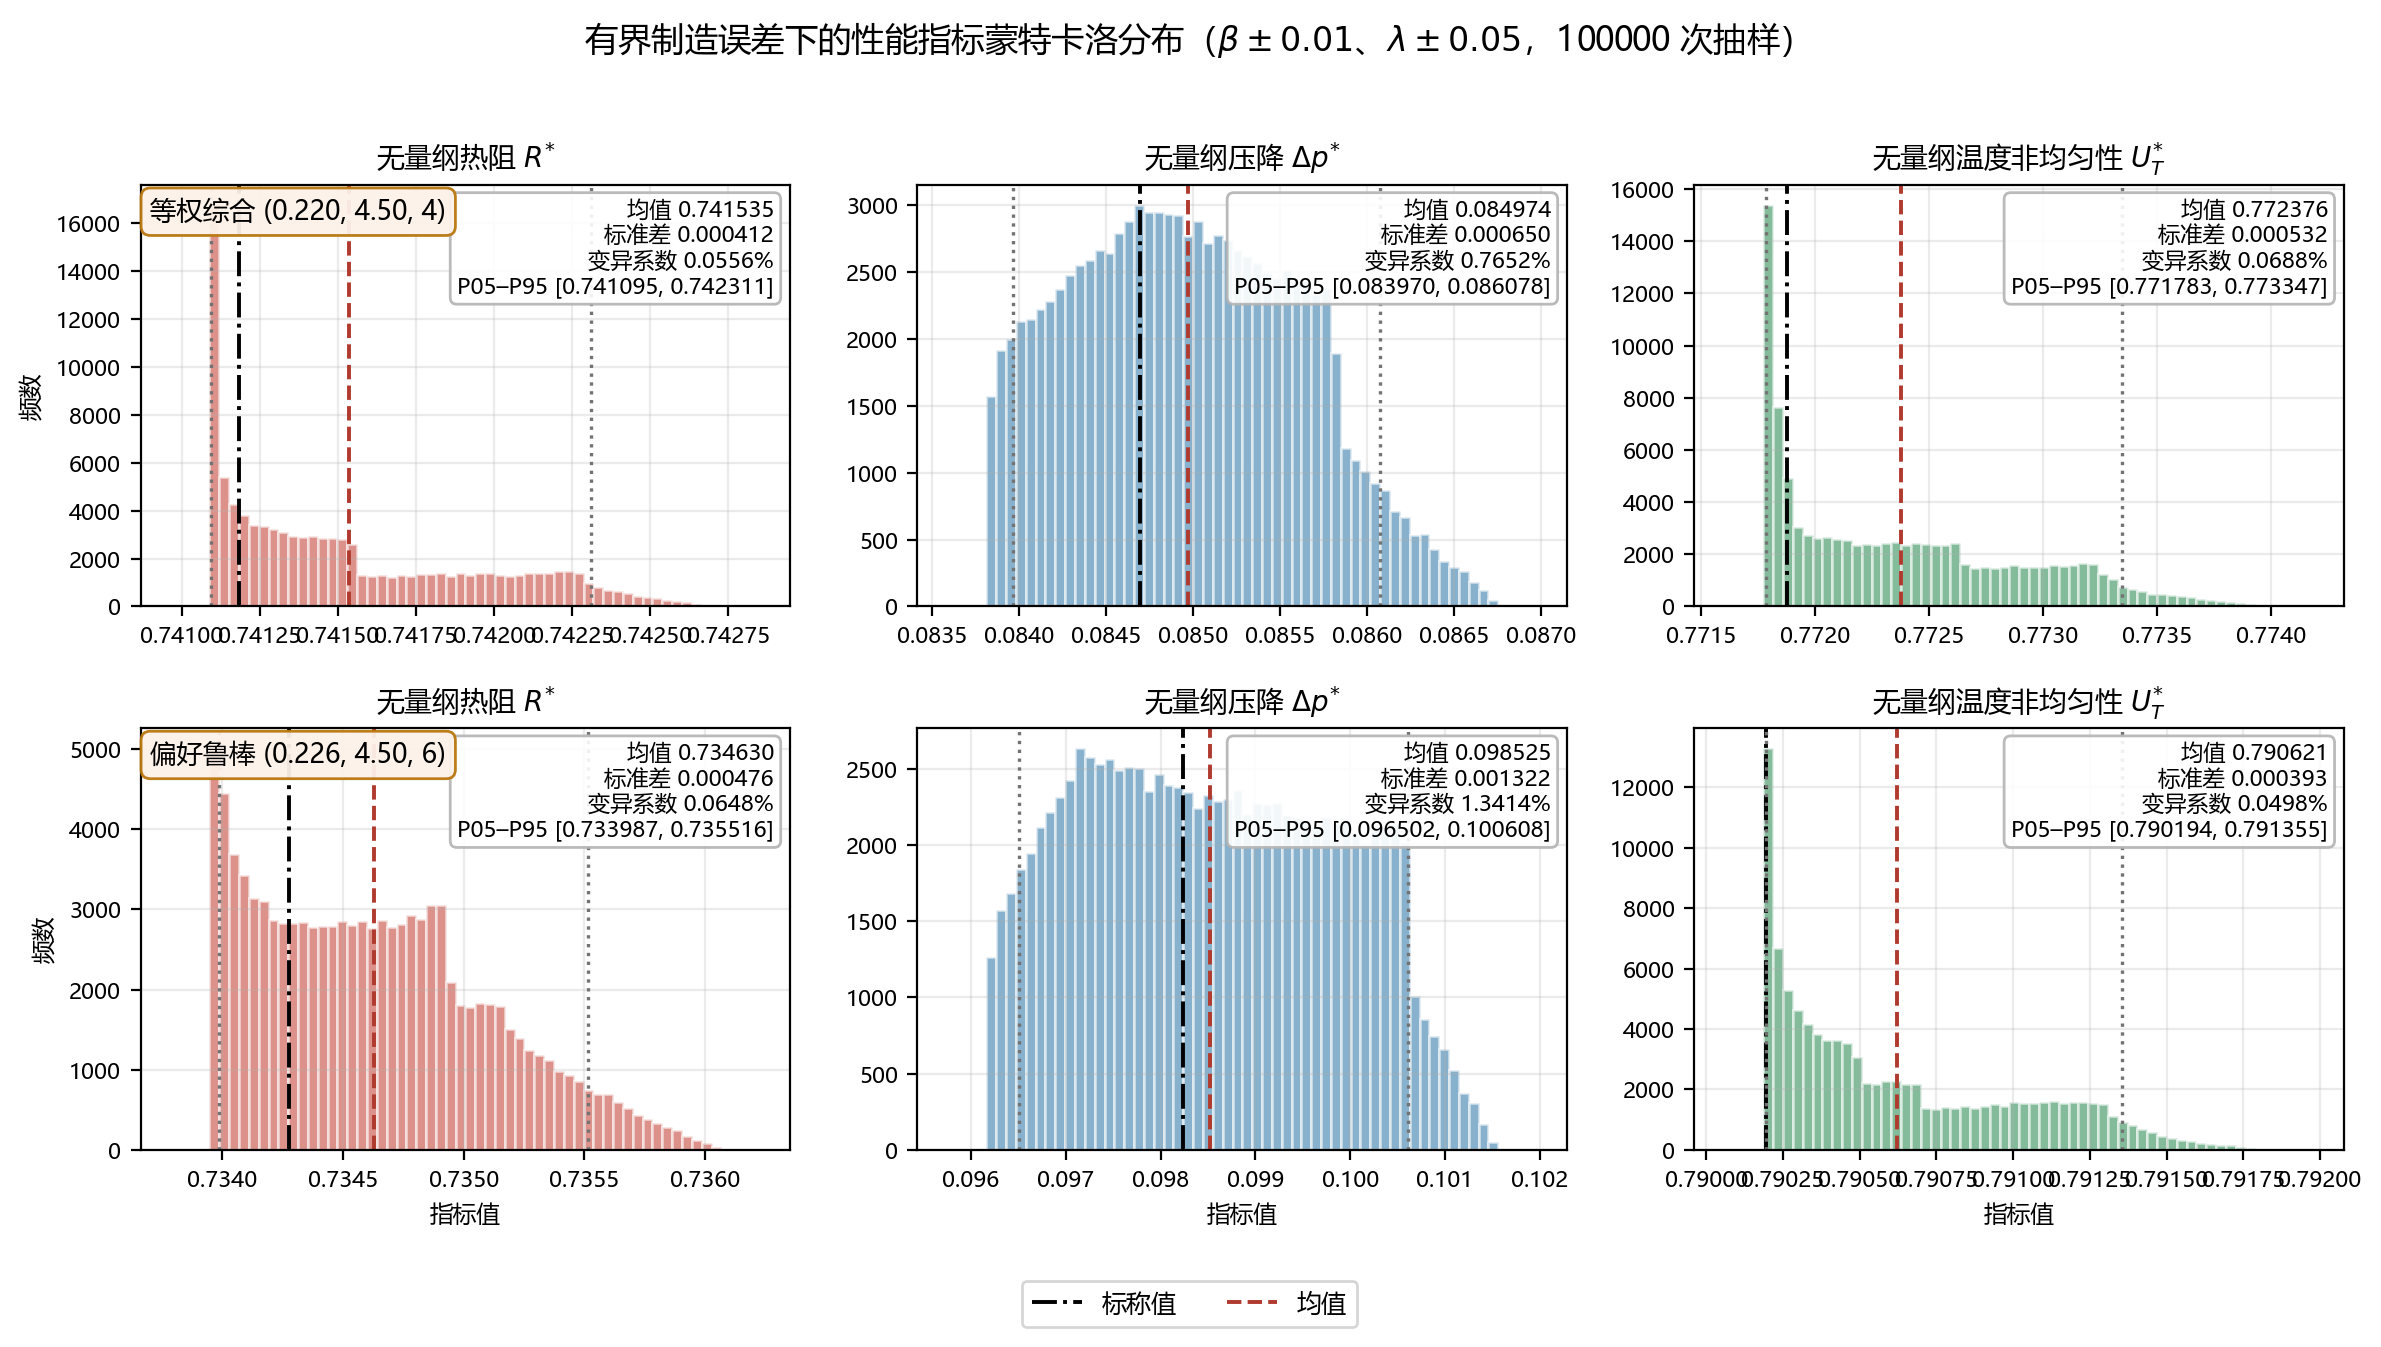
\includegraphics[width=0.94\textwidth]{figs/fig10_mc_hist.png}
  \caption{有界制造误差下两方案三项性能指标的蒙特卡洛分布（$\beta \pm 0.01$、$\lambda \pm 0.05$，100000 次抽样）}
  \label{fig:mc}
\end{figure}

\subsect{5.5.3\quad 针肋排数的离散扰动}
\begin{table}[htbp]
  \centering
  \caption{不同标称设计及针肋排数下的性能指标对比}
  \label{tab:nrows}
  \begin{tabular}{lcccc}
    \toprule
    标称设计 $(\beta, \lambda)$ & 排数 $N$ & 热阻 & 压降 & 温度非均匀性 \\
    \midrule
    等权参数 (0.220, 4.50) & 2 & 0.759836 & 0.076130 & 0.779056 \\
    等权参数 (0.220, 4.50) & 4 & 0.741183 & 0.084698 & 0.771878 \\
    等权参数 (0.220, 4.50) & 6 & 0.734634 & 0.096961 & 0.790285 \\
    鲁棒参数 (0.226, 4.50) & 4 & 0.741097 & 0.085343 & 0.771784 \\
    鲁棒参数 (0.226, 4.50) & 6 & 0.734274 & 0.098231 & 0.790195 \\
    鲁棒参数 (0.226, 4.50) & 8 & 0.734383 & 0.109646 & 0.812385 \\
    \bottomrule
  \end{tabular}
\end{table}
从 4 排增至 6 排，热阻下降，但压降和非均匀性明显上升；从 6 排增至 8 排，热阻几乎不再改善，而水力和均匀性代价继续增大。因此 4—6 排是有效折中区，8 排以上缺乏综合优势。

\subsect{5.5.4\quad 工况波动的可识别边界}
附件所有样本均固定在同一质量流量、入口温度和热源条件，代理模型没有学习 $\dot m$、$T_{\mathrm{in}}$、$q'''$ 三个工况维度。对压降只能由机理给出边界：黏性层流主导时 $\Delta p \propto \dot m$，局部惯性主导时近似 $\Delta p \propto \dot m^{2}$。若流量增加 5\%，则：
\begin{equation}
  \frac{\Delta p}{\Delta p_0} \in \left[\,1.05,\ 1.05^{2}\,\right] = \left[\,1.05,\ 1.1025\,\right].
  \label{eq:50}
\end{equation}
热阻和温度非均匀性对工况的数值响应无法由现有 84 点可靠识别。实际工程扩展应对 $\dot m$、$T_{\mathrm{in}}$、$q'''$ 各增加至少三个水平，将代理模型扩展为：
\begin{equation}
  \hat y = \Phi(\beta,\ \lambda,\ N,\ \dot m,\ T_{\mathrm{in}},\ q''').
  \label{eq:51}
\end{equation}
在没有新增 CFD 或实验数据前，本文不报告伪精确的工况扰动结果。

\subsect{5.6\quad 结论}
\begin{enumerate}[leftmargin=2.5em,itemsep=0pt]
  \item 结构参数通过``歧管压力分配—支路流量—针肋间隙速度—局部换热—温度场''链条影响性能。针肋宽度比和排数体现换热强化与流动阻塞的竞争；歧管深高比对压降显著有利，但对热阻和均匀性存在间接权衡。
  \item 带针肋域的三次响应面在重复交叉验证中达到 $R^{2} > 0.9995$，三项范围归一化 RMSE 均小于 0.47\%，能够支撑附件域内优化。无针肋结构因拓扑不同而单独处理。
  \item 等权综合推荐为 $(0.220, 4.50, 4)$，预测性能为 $(0.741183, 0.084698, 0.771878)$。理想点距离准则给出相邻的 6 排方案，交叉验证了 $\beta \approx 0.22$、$\lambda = 4.5$、$N = 4$—6 的折中区。
  \item 权重未知时，最小最大后悔方案为 $(0.226, 4.50, 6)$，最大后悔值为 0.270865。它并非三指标逐项支配等权方案，而是在偏好切换下更稳健。
  \item 在 $\beta \pm 0.01$、$\lambda \pm 0.05$ 的声明公差下，两方案三项指标变异系数均小于 1.34\%；偏好鲁棒方案的压降对针肋宽度更敏感，证明偏好鲁棒与制造稳健需要分别评价。
\end{enumerate}

% ==================== 六、模型的评价、改进与推广 ====================
\sect{六、模型的评价、改进与推广}
\subsect{6.1\quad 模型优点}
\begin{itemize}[leftmargin=2.5em,itemsep=0pt]
  \item 物理与数据闭环。守恒方程、水力网络和 NTU 换热关系解释变量作用，响应面只承担附件缺失闭合关系的数值识别。
  \item 尊重几何拓扑。无针肋基准与带针肋域条件建模，避免在不存在的 $\beta = 0$、$N > 0$ 结构上插值。
  \item 验证与优化分离。以重复交叉验证选择模型，再进行确定性全域网格搜索，降低过拟合和随机初值风险。
  \item 区分两类鲁棒性。最小最大后悔处理评价偏好不确定性，蒙特卡洛处理制造误差；二者没有被混为同一个``鲁棒''概念。
  \item 边界透明。排数保持离散，连续扰动不超出样本域，固定工况下不虚构流量或热负荷响应。
\end{itemize}
\subsect{6.2\quad 模型局限}
\begin{itemize}[leftmargin=2.5em,itemsep=0pt]
  \item 通道完整尺寸、针肋节距及原始无量纲定义缺失，无法以 CFD 独立复算每个样本。
  \item 无针肋组只有 4 点，其基准曲线不具备强外推能力。
  \item 推荐深高比位于 $\lambda = 4.5$ 上边界，说明样本域可能截断了进一步降压的趋势；是否继续加深必须新增结构点并同时核查体积与加工约束。
  \item 制造公差为情景假设，不是设备实测分布。进入工程设计后应以真实公差、相关性和工况概率替换均匀分布。
  \item 支持型 Pareto 集由加权和生成，非凸前沿上的非支持解可能被遗漏；现有结论适用于扫描所得候选集。
\end{itemize}
\subsect{6.3\quad 分层推荐}
常规综合设计：当三项指标没有明确优先级时，推荐：
\begin{equation}
  (\beta,\ \lambda,\ N) = (0.220,\ 4.50,\ 4).
  \label{eq:52}
\end{equation}
它具有最低附近的温度非均匀性和较低压降，在假设制造误差下压降变异系数为 0.765\%。

偏好未知设计：当产品应用尚未确定，未来可能在热阻、泵功和均匀性之间切换重点时，推荐：
\begin{equation}
  (\beta,\ \lambda,\ N) = (0.226,\ 4.50,\ 6).
  \label{eq:53}
\end{equation}
它牺牲部分压降和均匀性，以较低热阻控制权重变化下的最坏后悔；但应加强针肋宽度公差控制。

进一步验证重点：在 $\lambda = 4.5$ 附近加密 CFD/实验点，并新增 $\lambda > 4.5$ 但满足体积约束的结构；围绕 $\beta = 0.22$、$N = 4$、6 进行流量和热负荷多水平试验；同时输出原始温度场和支路流量，以直接验证 $C_m$ 与 $U_T$ 的关系。

% ==================== 七、参考文献 ====================
\sect{七、参考文献}
\begingroup
\small
\setlength{\parindent}{0pt}
\setlength{\parskip}{3pt}
\newcommand{\refitem}[1]{\par\hangindent=2em\hangafter=1 #1}
\refitem{[1] Cang D, Dong Z, Lv S, et al. Design and intelligent optimization of TSV-based embedded microchannel heatsinks in 2.5D Packaging[J]. International Journal of Heat and Mass Transfer, 2026, 255: 127908.}
\refitem{[2] Zhang J, Sadiqbatcha S, Tan S X D. Hot-trim: Thermal and reliability management for commercial multicore processors considering workload dependent hot spots[J]. IEEE Transactions on Computer-Aided Design of Integrated Circuits and Systems, 2022, 42(7): 2290-2302.}
\refitem{[3] He W, Yin E, Zhou F, et al. Integrated manifold microchannels and near-junction cooling for enhanced thermal management in 3D heterogeneous packaging technology[J]. Energy, 2024, 305: 132263.}
\refitem{[4] Tuckerman D B, Pease R F W. High-performance heat sinking for VLSI[J]. IEEE Electron Device Letters, 1981, 2(5): 126-129.}
\refitem{[5] Harpole G M, Eninger J E. Micro-channel heat exchanger optimization[C]//Proceedings of the Seventh Annual IEEE Semiconductor Thermal Measurement and Management Symposium. Phoenix, AZ: IEEE, 1991: 59-63.}
\refitem{[6] Kandlikar S G, Grande W J. Evolution of microchannel flow passages---thermohydraulic performance and fabrication technology[J]. Heat Transfer Engineering, 2003, 24(1): 3-17.}
\refitem{[7] Peles Y, Koşar A, Mishra C, et al. Forced convective heat transfer across a pin fin micro heat sink[J]. International Journal of Heat and Mass Transfer, 2005, 48(17): 3615-3627.}
\refitem{[8] Drummond K P, Back D, Sinanis M D, et al. A hierarchical manifold microchannel heat sink array for high-heat-flux two-phase cooling of electronics[J]. International Journal of Heat and Mass Transfer, 2018, 117: 319-330.}
\refitem{[9] Bergman T L, Lavine A S, Incropera F P, et al. Fundamentals of Heat and Mass Transfer[M]. 7th ed. Hoboken: John Wiley \& Sons, 2011.}
\refitem{[10] Box G E P, Draper N R. Response Surfaces, Mixtures, and Ridge Analyses[M]. 2nd ed. Hoboken: John Wiley \& Sons, 2007.}
\refitem{[11] Rasmussen C E, Williams C K I. Gaussian Processes for Machine Learning[M]. Cambridge, MA: MIT Press, 2006.}
\refitem{[12] Deb K, Pratap A, Agarwal S, et al. A fast and elitist multiobjective genetic algorithm: NSGA-II[J]. IEEE Transactions on Evolutionary Computation, 2002, 6(2): 182-197.}
\refitem{[13] Savage L J. The theory of statistical decision[J]. Journal of the American Statistical Association, 1951, 46(253): 55-67.}
\refitem{[14] Metropolis N, Ulam S. The Monte Carlo method[J]. Journal of the American Statistical Association, 1949, 44(247): 335-341.}
\endgroup

% ==================== 附录 ====================
\sect{附录}
\subsect{附录 A\quad 三次响应面回归系数}
表 \ref{tab:coef} 给出带针肋域三次响应面（式（\ref{eq:35}））在三项指标上的回归系数。所有系数对应标准化变量 $z_\beta$、$z_\lambda$、$z_N$（式（\ref{eq:36}）），拟合采用 $\alpha = 10^{-10}$ 的 Ridge 正则，可据此直接复现正文全部预测结果。

\begin{table}[htbp]
  \centering
  \caption{三次响应面回归系数（标准化变量）}
  \label{tab:coef}
  \footnotesize
  \begin{tabular}{lccc}
    \toprule
    项 & 无量纲热阻 $a(R^{*})$ & 无量纲压降 $a(\Delta p^{*})$ & 无量纲温度非均匀性 $a(U_T^{*})$ \\
    \midrule
    1 & 7.396330e-01 & 1.079398e-01 & 7.912094e-01 \\
zβ & -3.287263e-03 & 1.359525e-02 & 2.777832e-02 \\
zλ & 6.491055e-03 & -1.547318e-02 & 5.198946e-03 \\
zN & -9.217626e-03 & 9.023163e-03 & -1.349303e-02 \\
zβ² & 2.817848e-03 & -1.295312e-03 & 4.092053e-03 \\
zβzλ & -9.647714e-05 & -4.727210e-05 & 2.455184e-03 \\
zβzN & -2.089219e-03 & 3.966984e-03 & 6.693766e-03 \\
zλ² & -2.927153e-03 & 8.182709e-03 & 2.926351e-03 \\
zλzN & -8.422010e-04 & 3.182929e-05 & 2.304834e-03 \\
zN² & 4.661002e-03 & 5.343803e-03 & 8.109145e-03 \\
zβ³ & -2.453115e-03 & -2.391494e-03 & -1.032570e-02 \\
zβ²zλ & 2.914367e-03 & 3.234033e-04 & -7.047048e-04 \\
zβ²zN & 1.364948e-03 & 5.034821e-05 & 1.137779e-03 \\
zβzλ² & -2.573668e-03 & -1.039248e-03 & -6.387200e-03 \\
zβzλzN & 3.905684e-04 & -1.175191e-03 & 1.215329e-03 \\
zβzN² & -1.868588e-03 & -9.946328e-05 & -6.589713e-04 \\
zλ³ & -5.599623e-04 & -5.471582e-05 & -3.347728e-03 \\
zλ²zN & 9.879985e-04 & 2.093608e-03 & -1.146784e-03 \\
zλzN² & 5.689409e-04 & -1.449766e-04 & 2.038853e-03 \\
zN³ & 2.482947e-03 & 2.523120e-03 & 7.079985e-03
    \\
    \bottomrule
  \end{tabular}
\end{table}

\subsect{附录 B\quad 数值实验与复现说明}
\begin{itemize}[leftmargin=2.5em,itemsep=0pt]
  \item 数据来源：附件 2 共 84 组样本，其中带针肋 80 组（$\beta$、$\lambda$、$N$ 的 $4 \times 4 \times 5$ 完整因子设计），无针肋 4 组（$\beta = 0$、$N = 0$）。
  \item 代理模型：标准化三次响应面 + Ridge（$\alpha = 10^{-10}$）；5 次重复 5 折交叉验证（随机种子 6）；高斯过程采用 RBF 与 White 核组合。
  \item 优化搜索：$\beta$ 步长 0.001、$\lambda$ 步长 0.01、$N$ 枚举 5 个水平，共 151755 个带针肋方案；指标极值归一化采用全部 84 组样本；Pareto 候选由权重步长 0.05 的加权和扫描构造（115 个方案），后悔值在权重步长 0.01 的单纯形网格上评价。
  \item 蒙特卡洛传播：每方案 100000 次独立抽样（随机种子 31），$\beta$、$\lambda$ 分别取均匀分布并截断于设计域。全部计算基于 Python 3（NumPy、Pandas、scikit-learn、Matplotlib）实现，正文图表均可复现。
\end{itemize}

\end{document}
